\subsection{Notations}
\begin{wrapfigure}{r}{2.5in}
  \vspace{-50pt}
  \begin{center}
    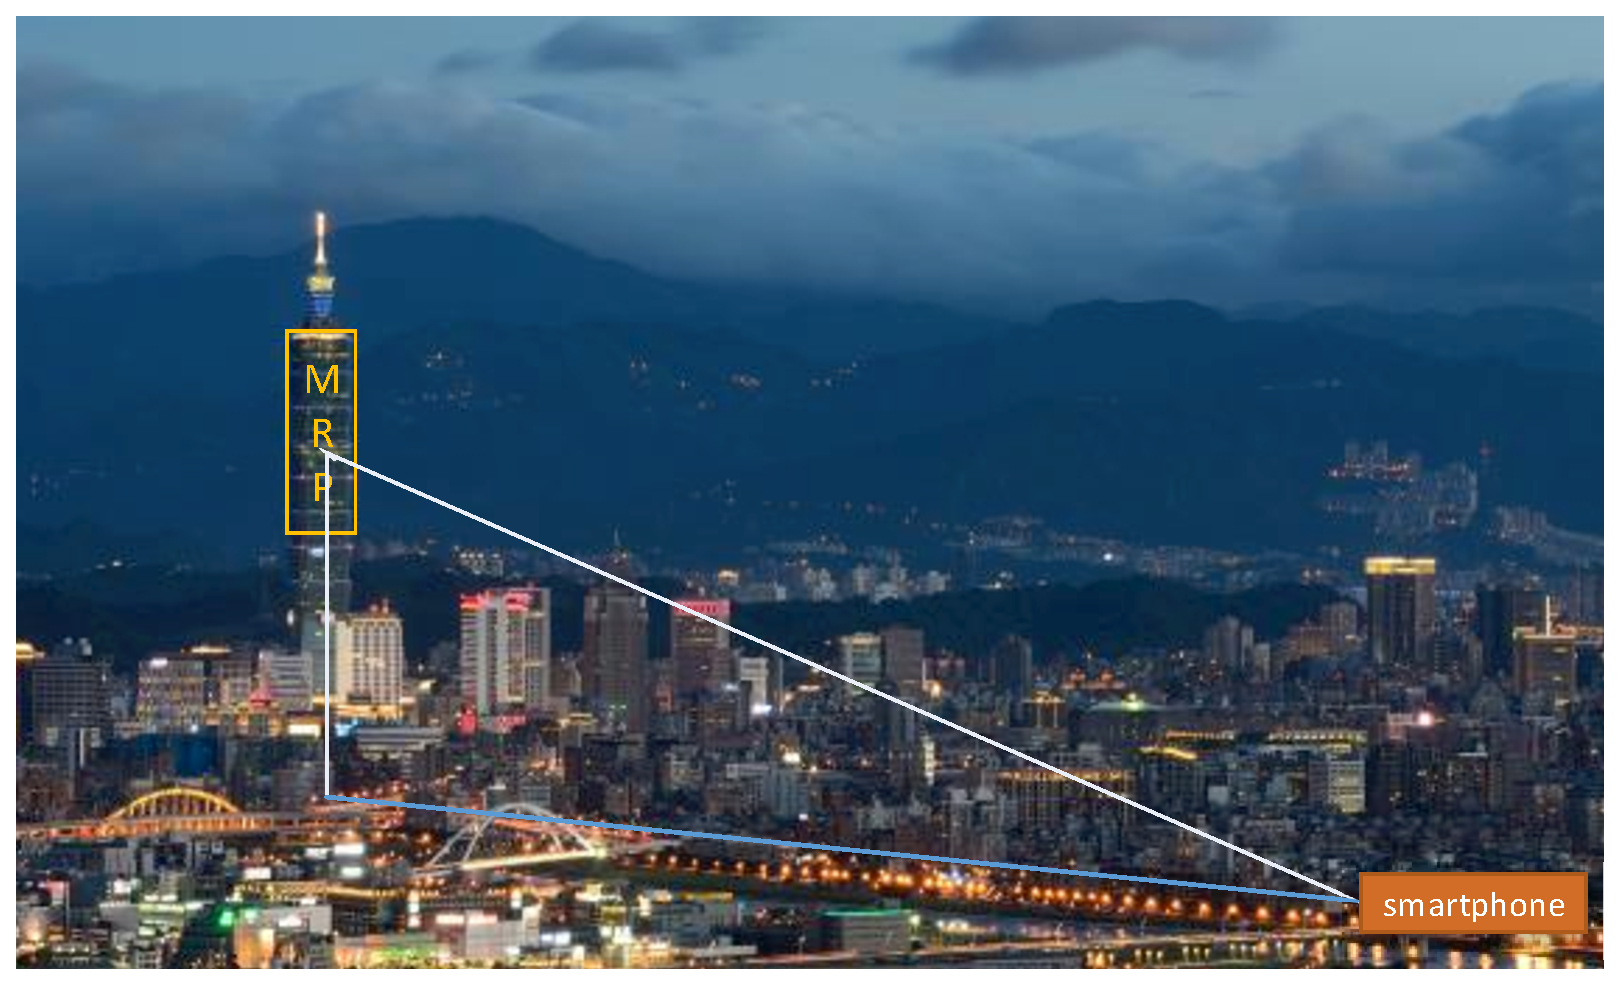
\includegraphics[width=2.5in]{fig/fig-taipei101.eps}
  \end{center}
  \vspace{-20pt}
  \caption{Schematic diagram (Using Taipei 101 as MRP)}\label{fig-taipei101}
  \vspace{-35pt}
\end{wrapfigure}
In the following, we summarize the notations used in the rest of the thesis.
\begin{mydef}
Angle of View: In photography, angle of view describes the angular extent of a given scene that is imaged by a camera. It is used interchangeably with the more general term field of view~\cite{wiki-angle-of-view}.
\end{mydef}
\begin{mydef}
Angle of Object: Angle of object describes the angular extent of a given object that is imaged by a camera. In our work. The angle of object is denoted as $\theta$, which is formed by the lines of the top of the object to the camera and the bottom of the object to the camera. Figure~\ref{fig-angle-of-view} illustrates an example of the angle of object.
\end{mydef}
%\begin{figure}
%  \centering
%  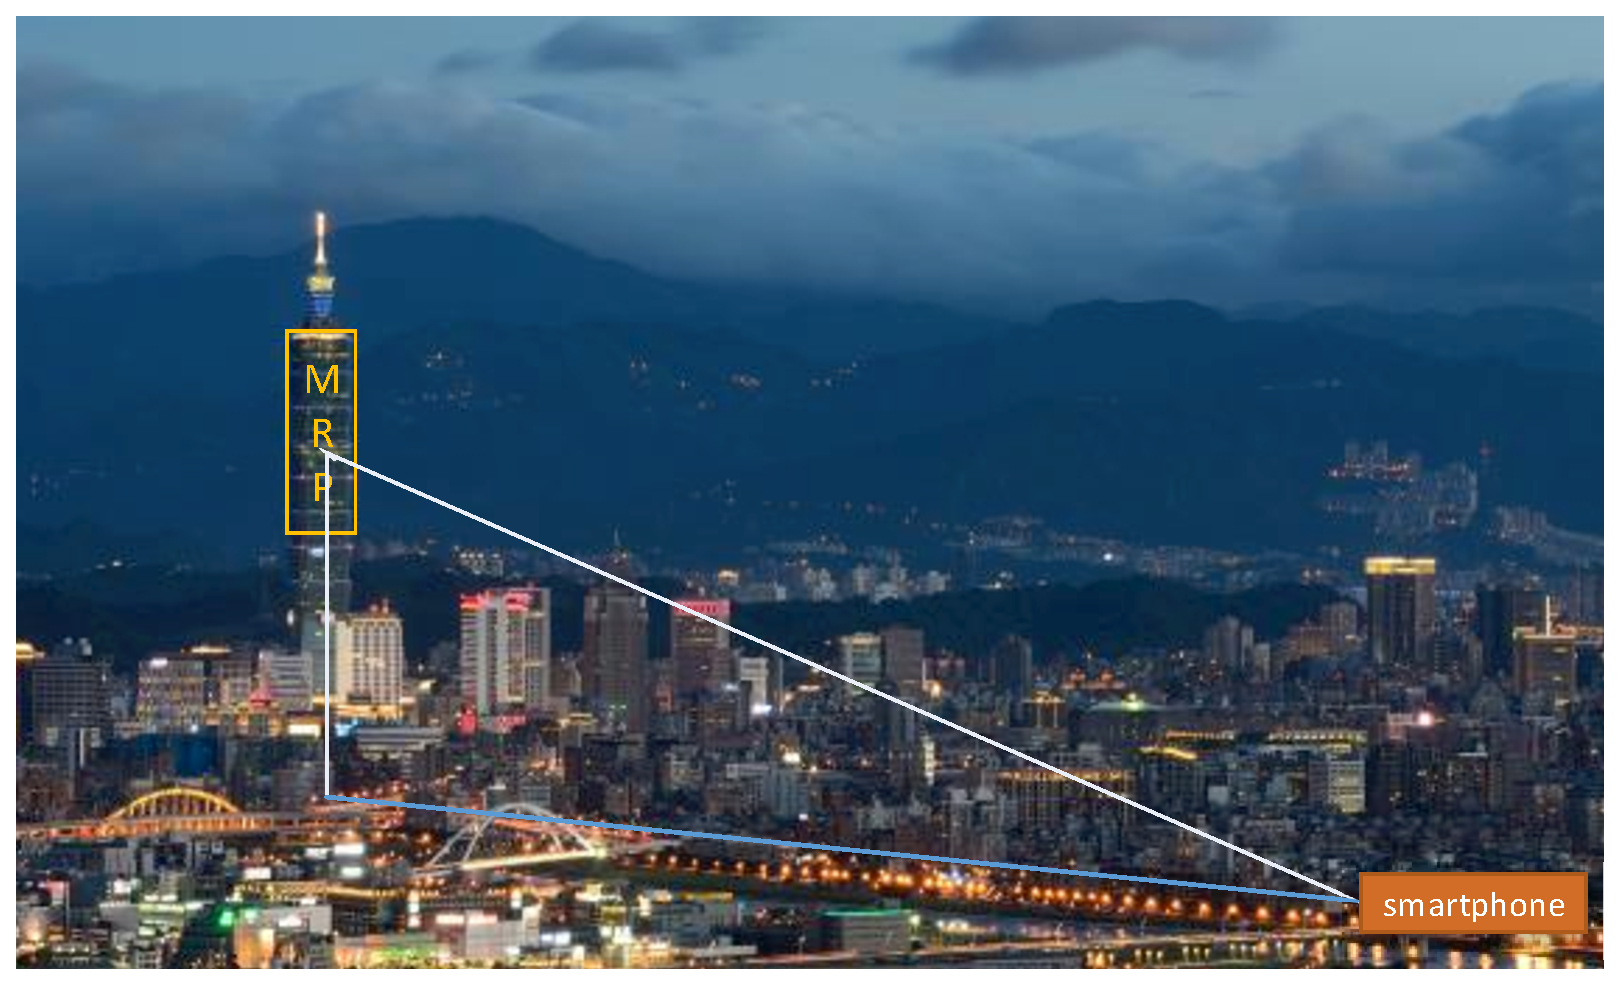
\includegraphics[width=3.3in]{fig/fig-taipei101.eps}\\
%  \caption{Schematic diagram (Using Taipei 101 as MRP)}\label{fig-taipei101}
%\end{figure}
%\begin{figure}
%  \centering
%  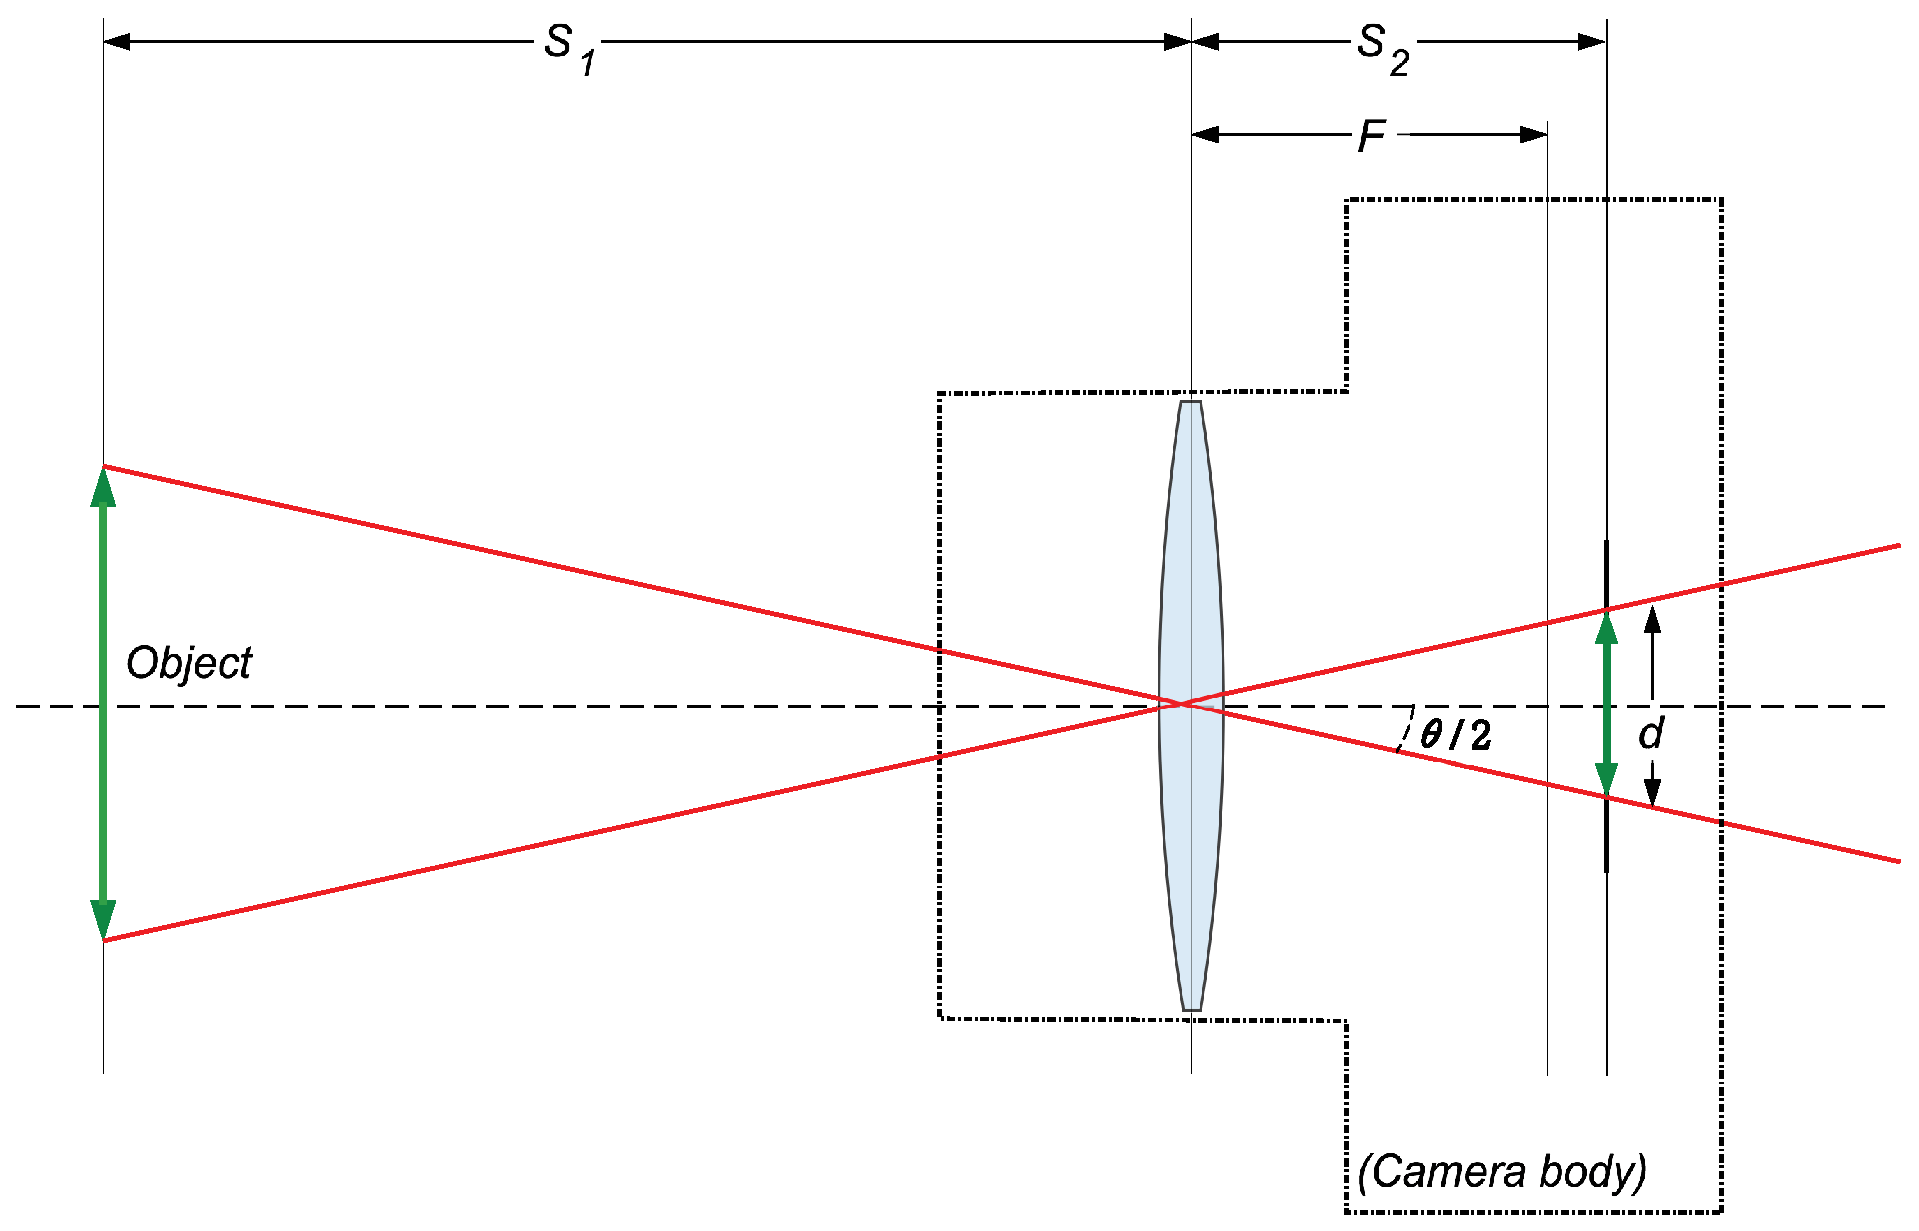
\includegraphics[width=3.5in]{fig/fig-angle-of-view.eps}\\
%  \caption{Angle of object.}\label{fig-angle-of-view}
%\end{figure}

\subsection{Measurable Reference Point (MRP)}
When we take a photo which contains an image of a known object, it is possible to derive our current position based on the size and angle of the image of the known object. For the ease of reference, in the rest of this thesis we refer to the known object in the photo as the \emph{Measurable Reference Point} (MRP). Basically, the location, orientation, and the size of the MRP is known in advance for reference. For instance, we know the exact location and the height of Taipei 101~\cite{wiki-taipei101}. If our photo contains the image of Taipei 101, we can use it as our MRP to infer our position at the time when the photo is taken.
Optical positioning systems that rely entirely on natural features in the images lack robustness, in particular under conditions with varying illumination. In order to increase robustness and improve accuracy of reference points, dedicated MRP are used for systems with demanding requirements for positioning. The MRP serves three purposes for the development of the positioning algorithm: First, it simplifies the automatic detection of corresponding points. Second, the shape, size, and location of MRP have to be known. Third, the MRP can be easily identified and is unique in the positioning environment. One good example of MRP for small and median-scale range is the QR-code, as it is easy to identify and is unique in the target environment.

\subsection{Angle Measurement}\label{sec-angle-measurement}
To calculate the angle of object, we first need to obtain the angle of view. The angle of view can be obtained directly from Android API by calling:
\begin{verbatim}
android.hardware.Camera.Parameters.getHorizontalViewAngle();
android.hardware.Camera.Parameters.getVerticalViewAngle();
\end{verbatim}

\begin{wrapfigure}{r}{2.3in}
  \vspace{-35pt}
  \begin{center}
    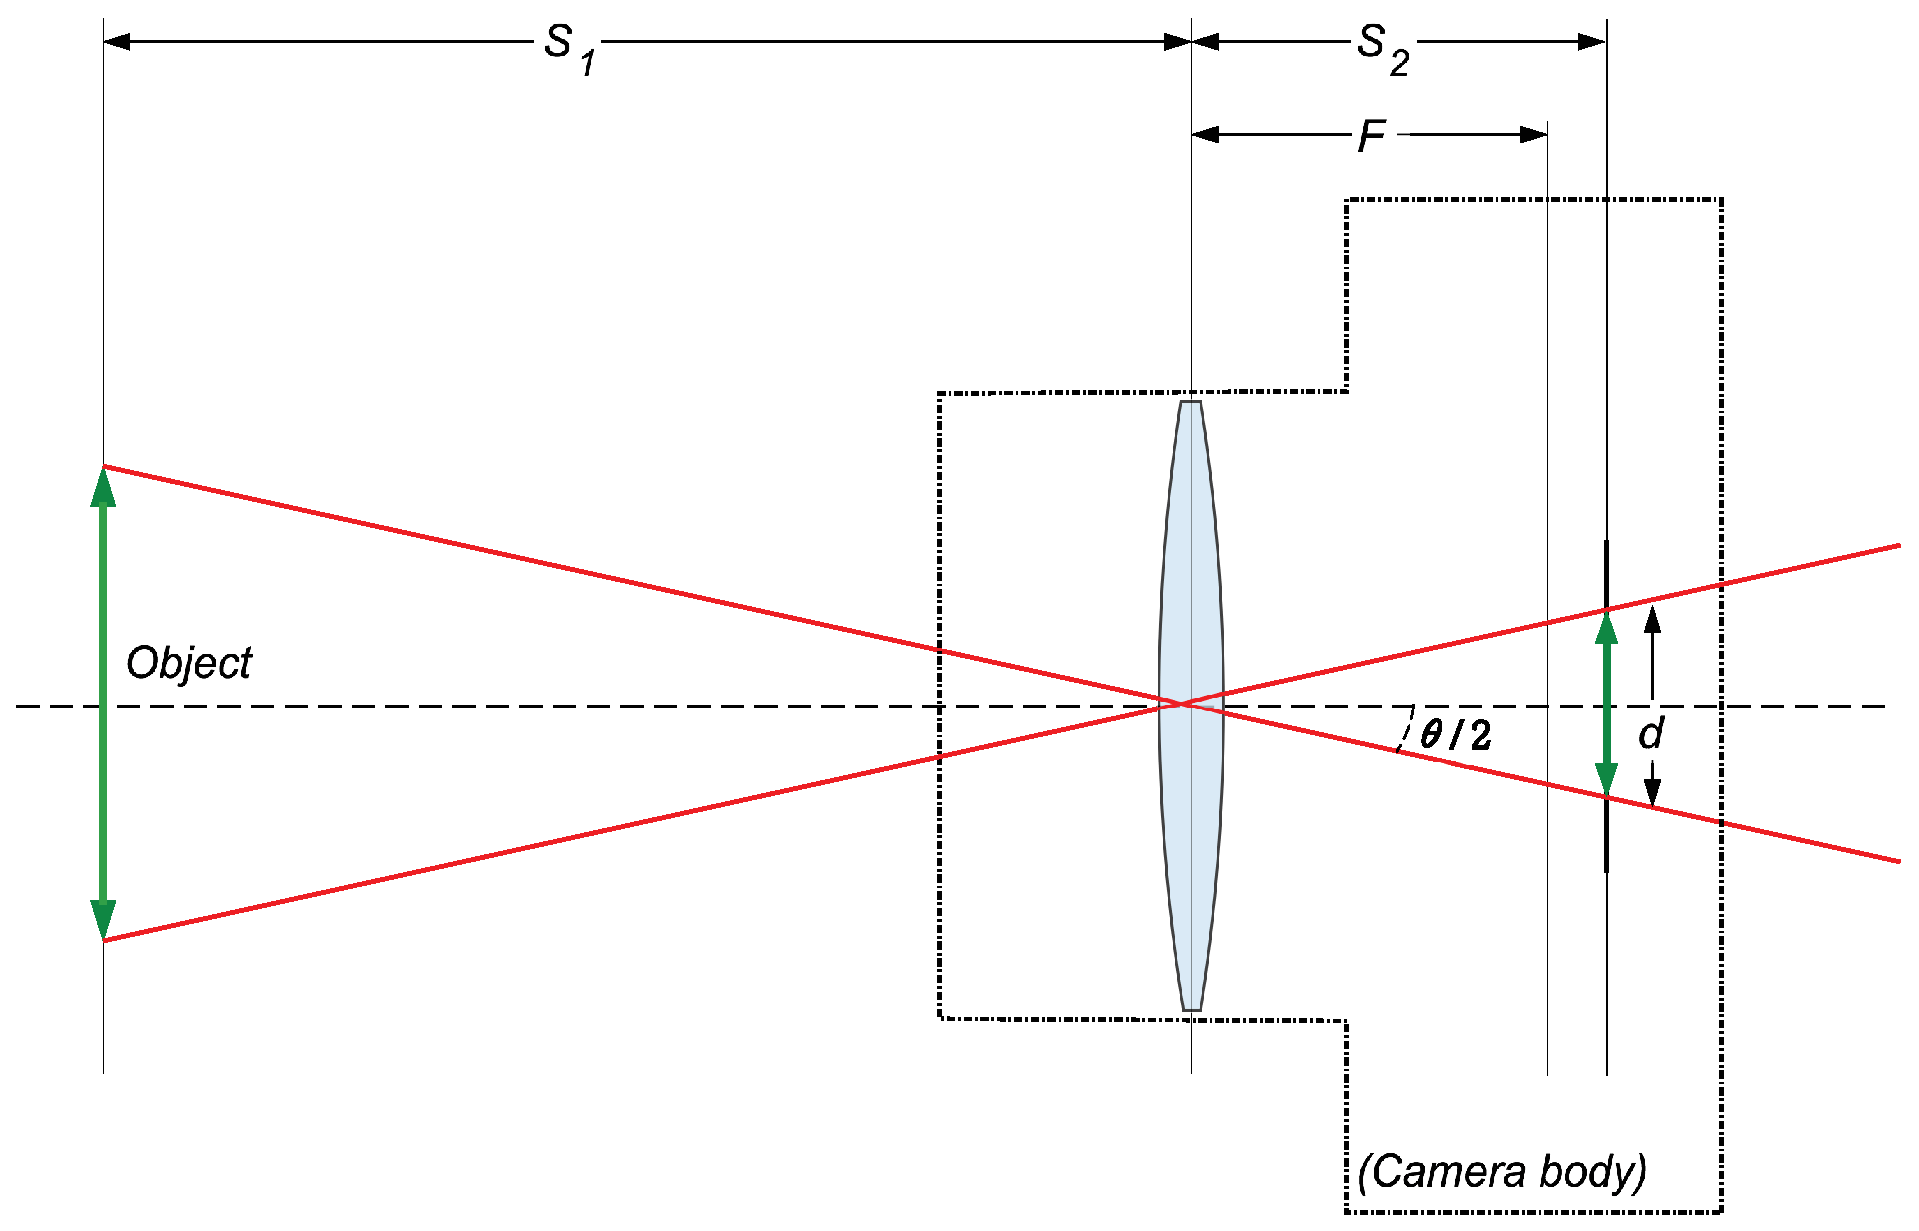
\includegraphics[width=2.5in]{fig/fig-angle-of-view.eps}
  \end{center}
  \vspace{-20pt}
  \caption{Angle of object.}\label{fig-angle-of-view}
  \vspace{-35pt}
\end{wrapfigure}

Here, we treat the lens as if it were a pinhole at distance $S_2$ from the image plane. We can obtain $S_2$ by the following equation.
\[tan(\frac{\theta}{2})=\frac{d/2}{S_2}\]

Note that once $S_2$ and the object size \emph{d} are acquired, the angle of object can be proportionally calculated by the following equation.
\[\theta=2arctan(\frac{d}{2S_2})\]

\subsection{Distance Measurement}

In our computation, we use triangle functions to measure the distance between MRP and the camera.
Based on the relative orientation of the object to the camera, we separate the distance measurement into three different cases.

\subsubsection{Basic Case}\label{sec-measure-distance-basic-case}

\begin{wrapfigure}{r}{2.3in}
  \vspace{-20pt}
  \begin{center}
    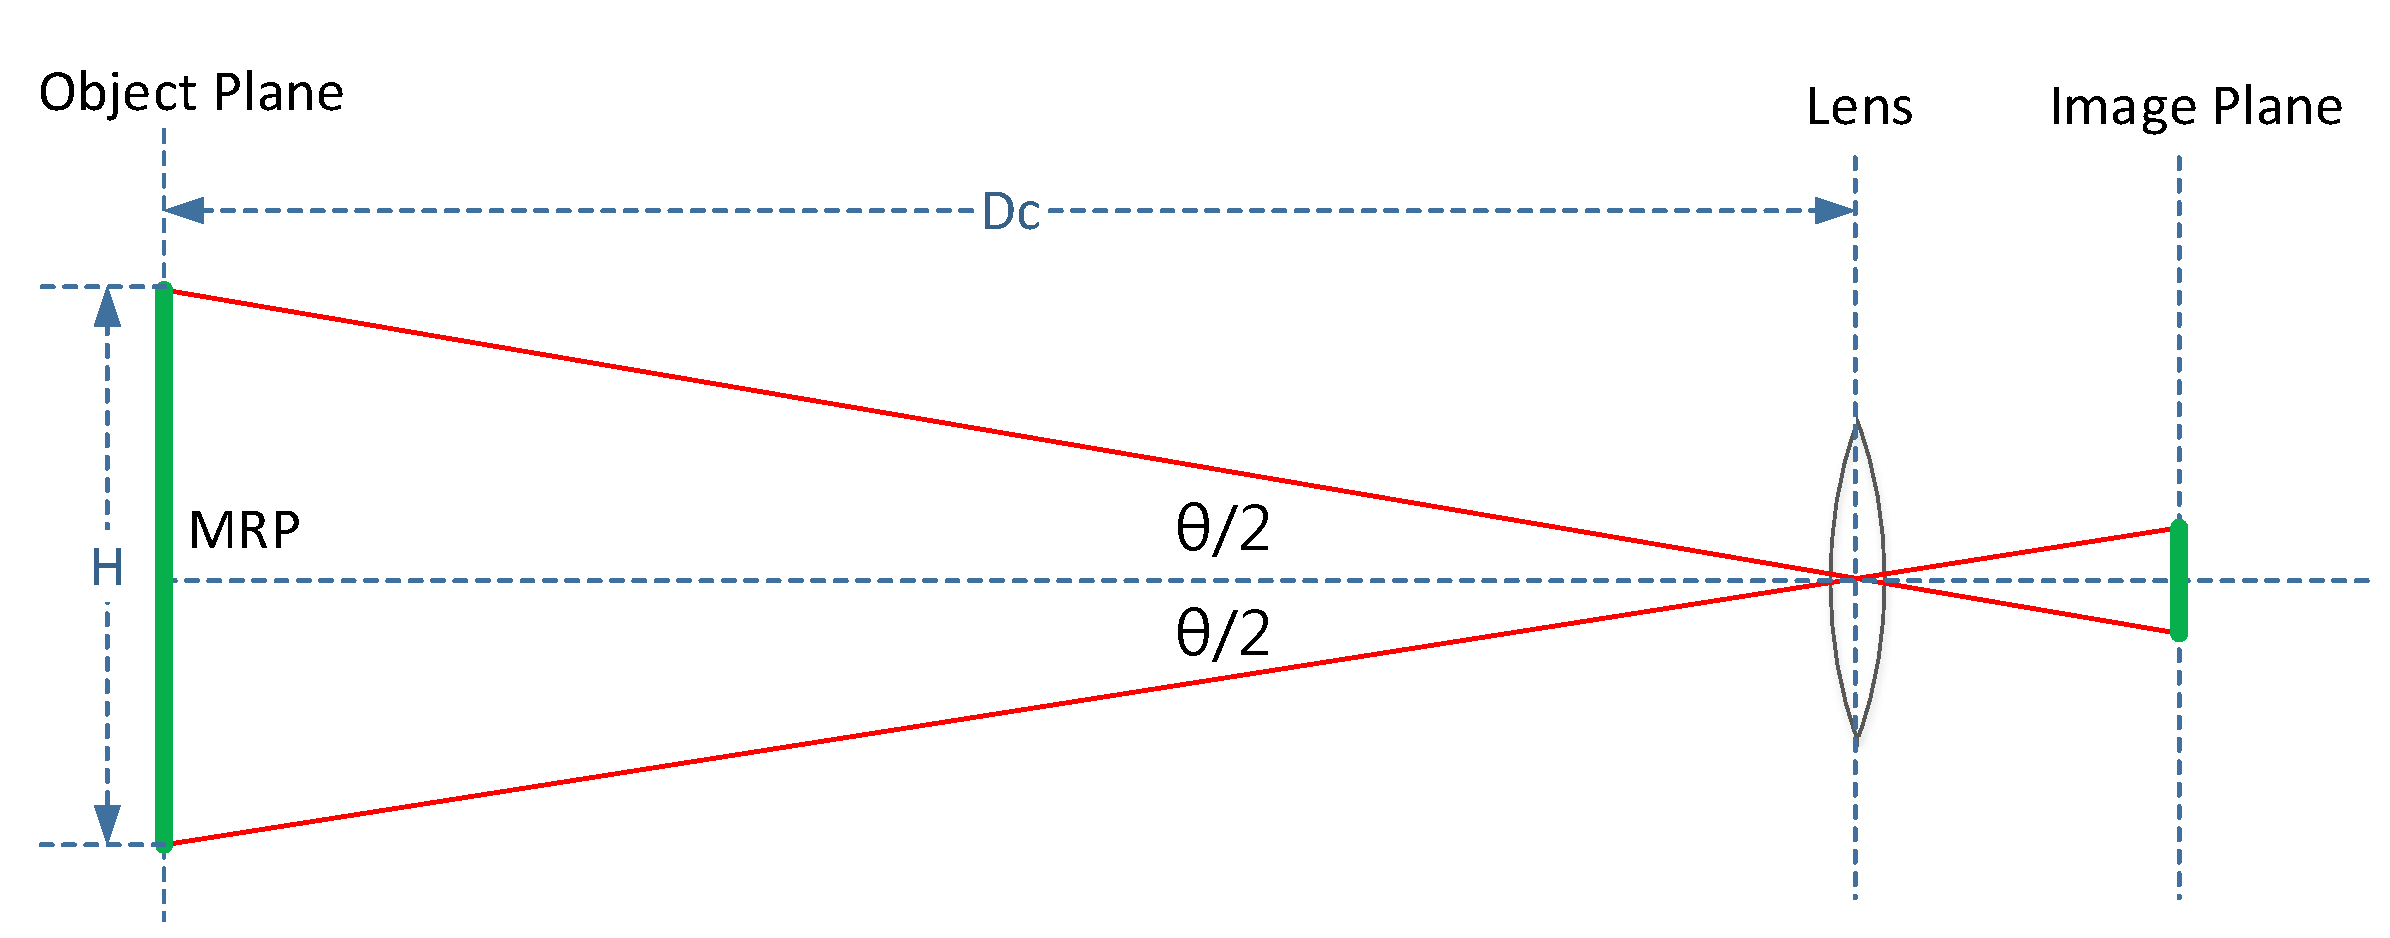
\includegraphics[width=2.5in]{fig/fig-distance-case1.eps}
  \end{center}
  \vspace{-20pt}
  \caption{Measure distance basic case.}\label{fig-distance-case1}
  \vspace{-20pt}
\end{wrapfigure}
%\begin{figure}
%  \centering
%  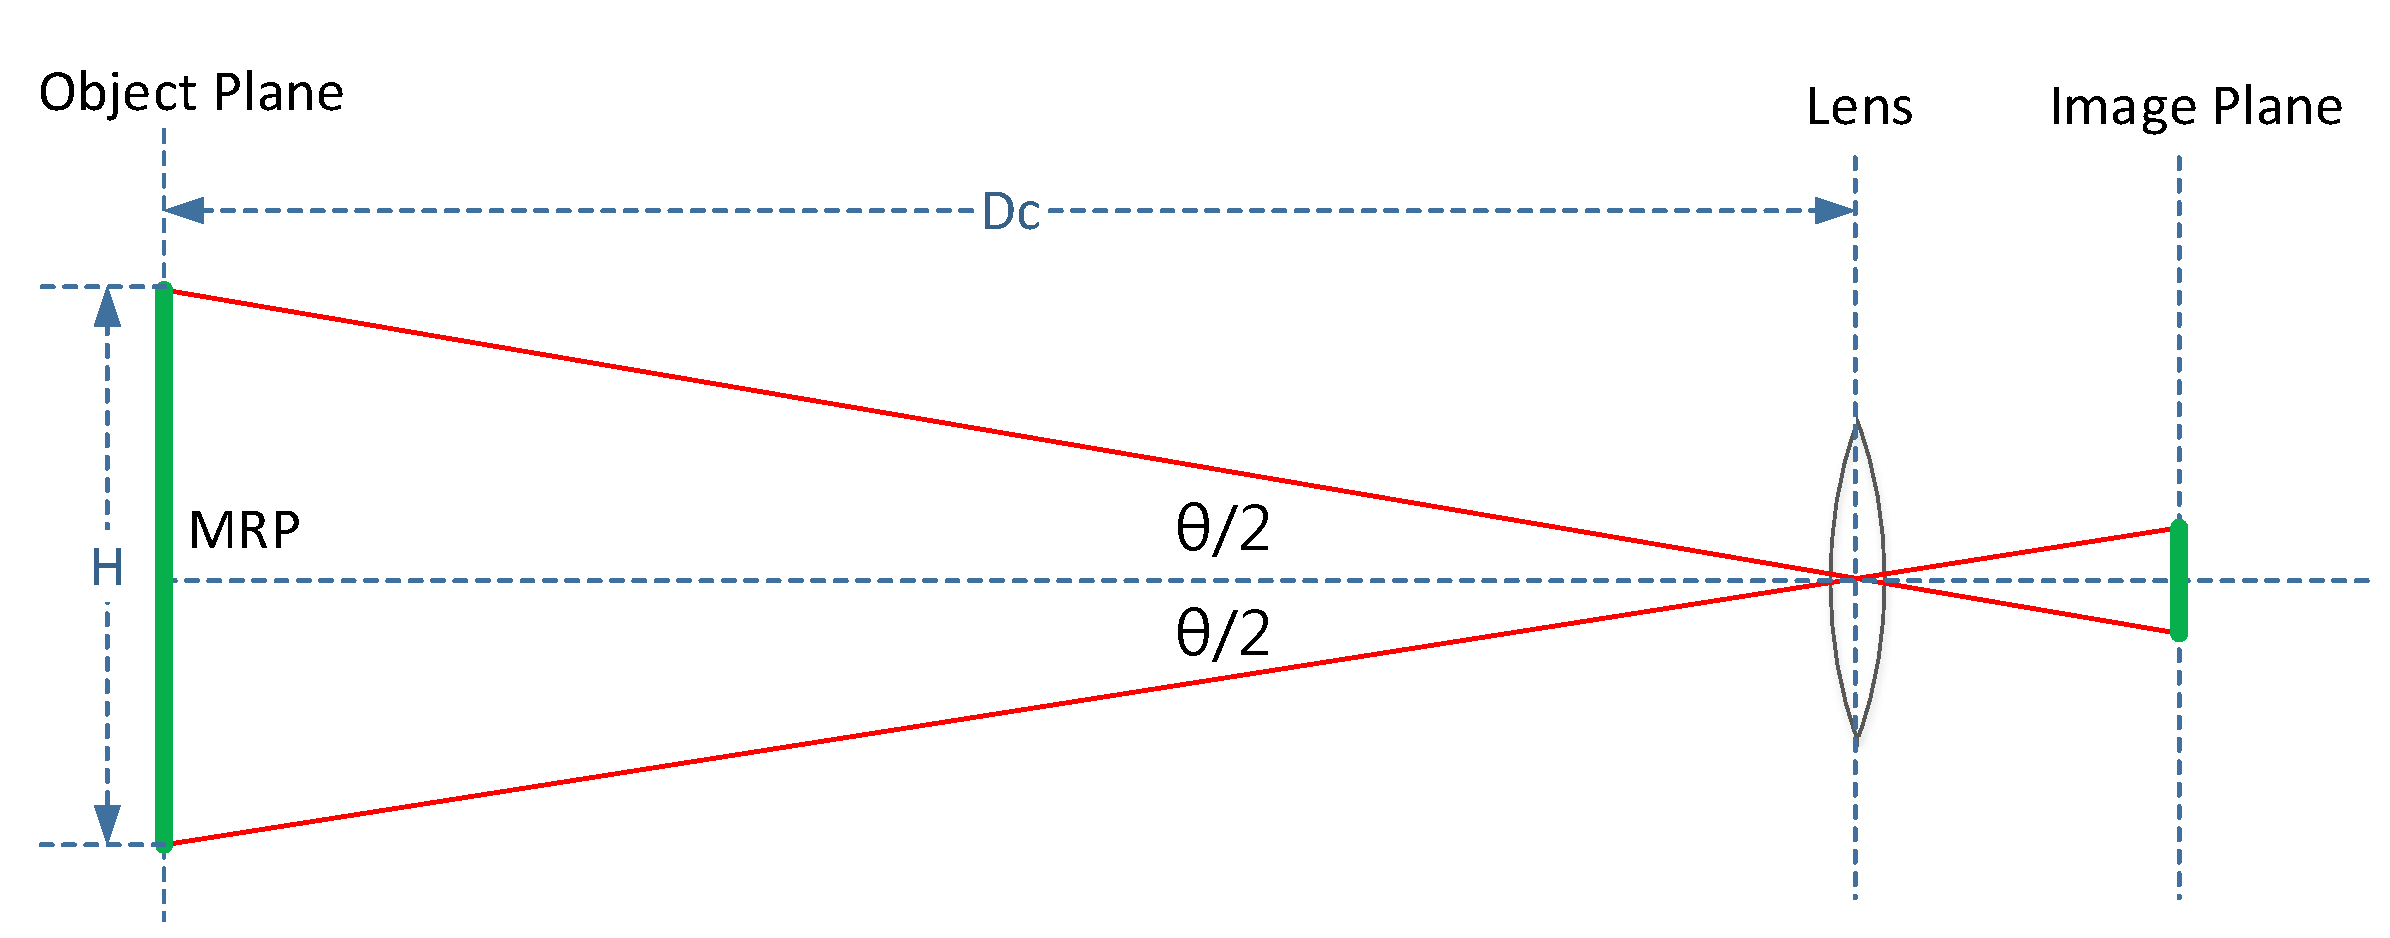
\includegraphics[width=3.5in]{fig/fig-distance-case1.eps}\\
%  \caption{Measure distance basic case.}\label{fig-distance-case1}
%\end{figure}
In this case. the MRP object is facing directly toward the center of the camera. Figure~\ref{fig-distance-case1} illustrates an example of this case. This is the simplest case for distance measurement. In addition to the size of MRP (denoted as \emph{H}), the additional required parameter of the camera for visual-based localization includes the view of angle for the object (denoted as $\theta$). We can use the method mentioned in Section~\ref{sec-angle-measurement} to calculate $\theta$. Once $\theta$ is obtained, the distance between MRP and camera can be computed by the following equation.

\[Dc = \frac{H}{2}/\tan (\frac{\theta }{2})\]

\subsubsection{MRP Shifted on Object Plane}
\begin{wrapfigure}{r}{2.3in}
  \vspace{-20pt}
  \begin{center}
    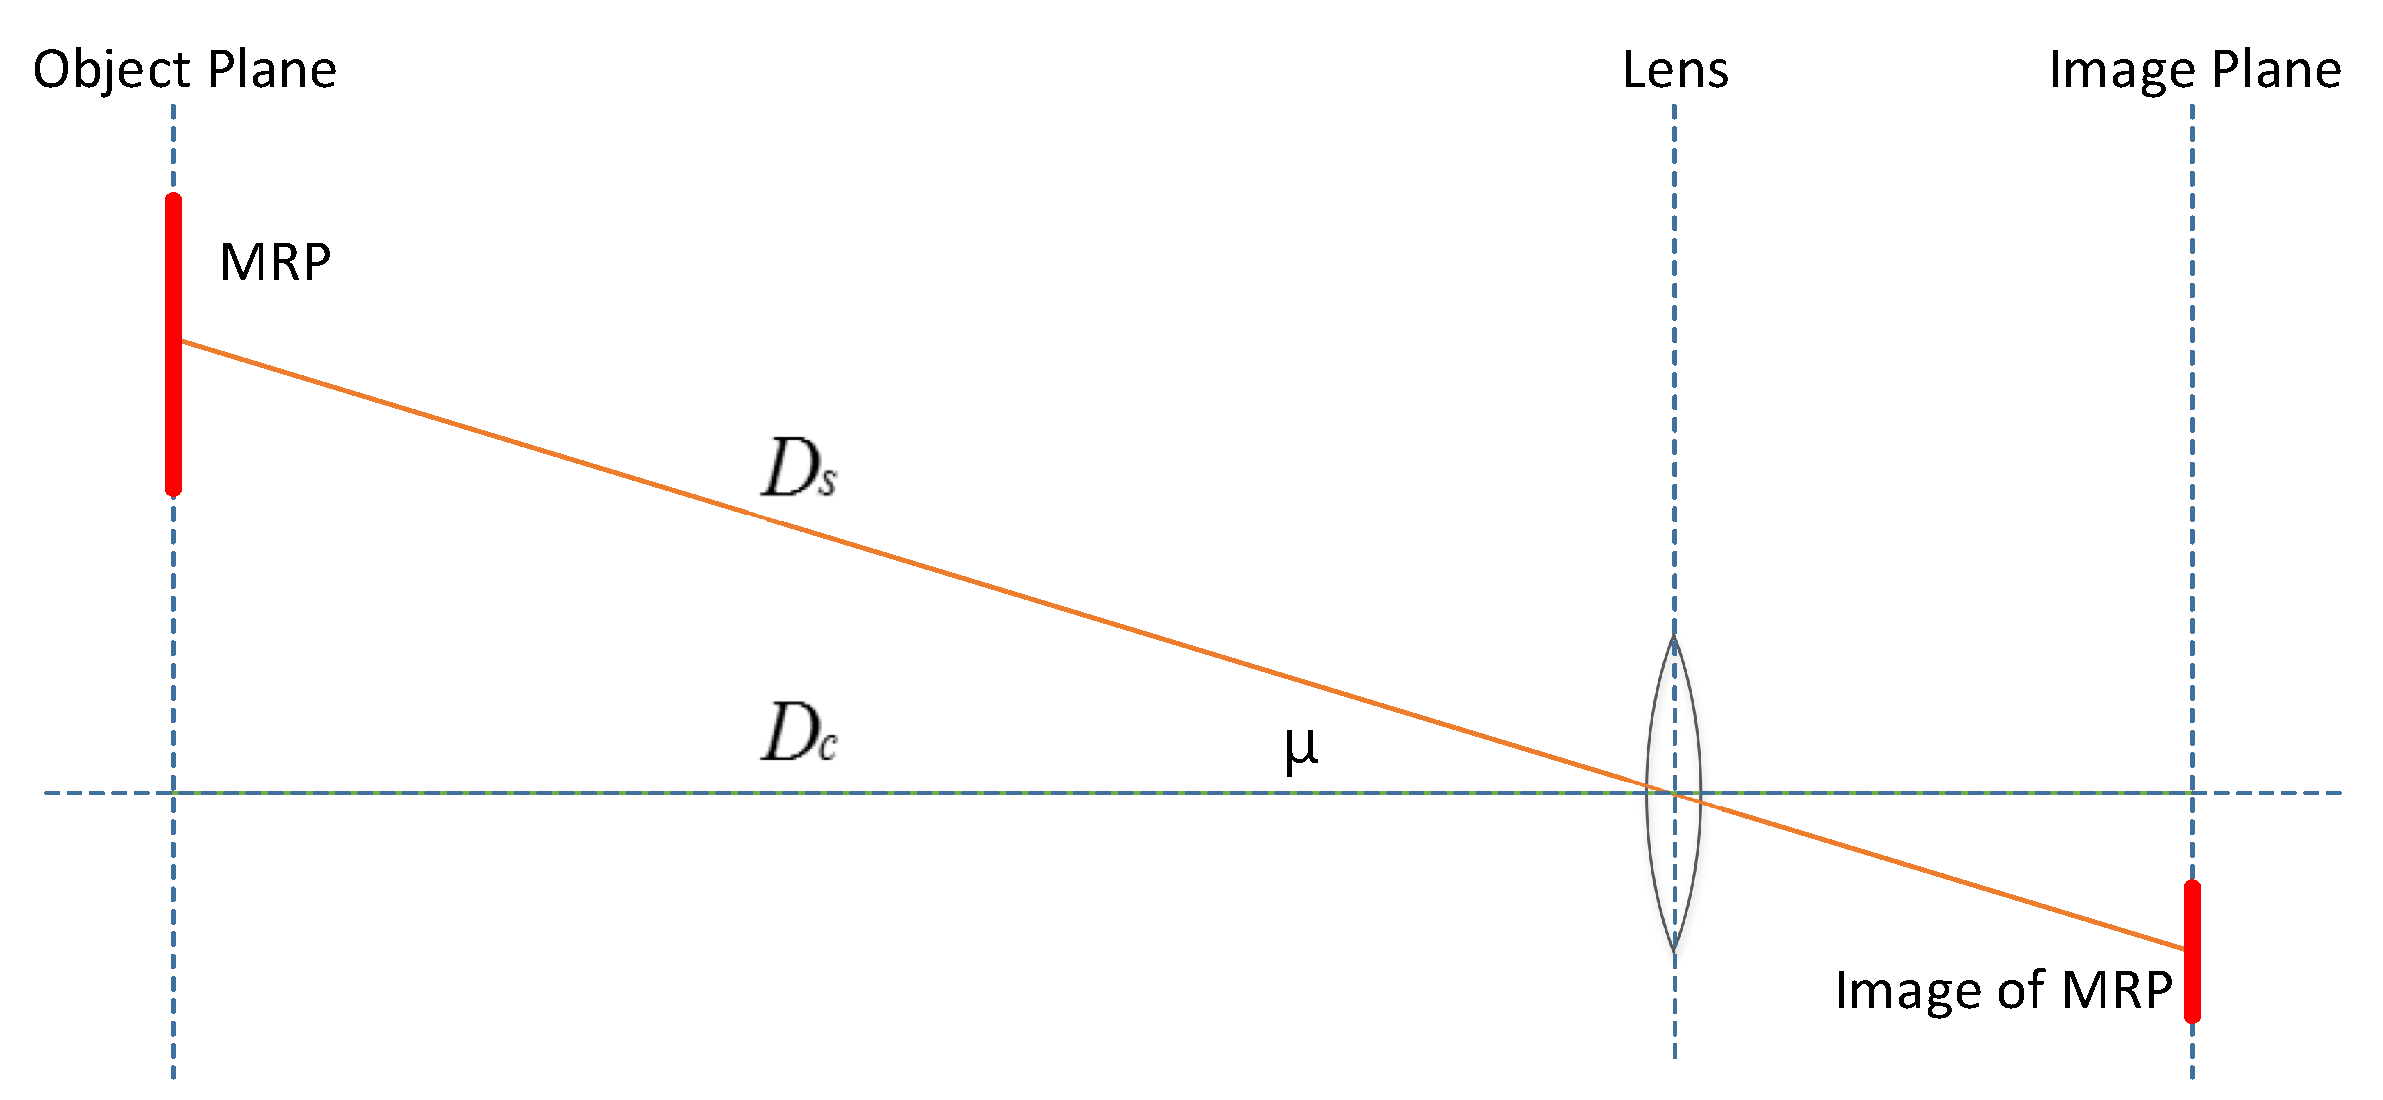
\includegraphics[width=2.5in]{fig/fig-distance-case2.eps}
  \end{center}
  \vspace{-20pt}
  \caption{MRP shifted on object plane.}\label{fig-distance-case2}
  \vspace{-20pt}
\end{wrapfigure}
%\begin{figure}
%  \centering
%  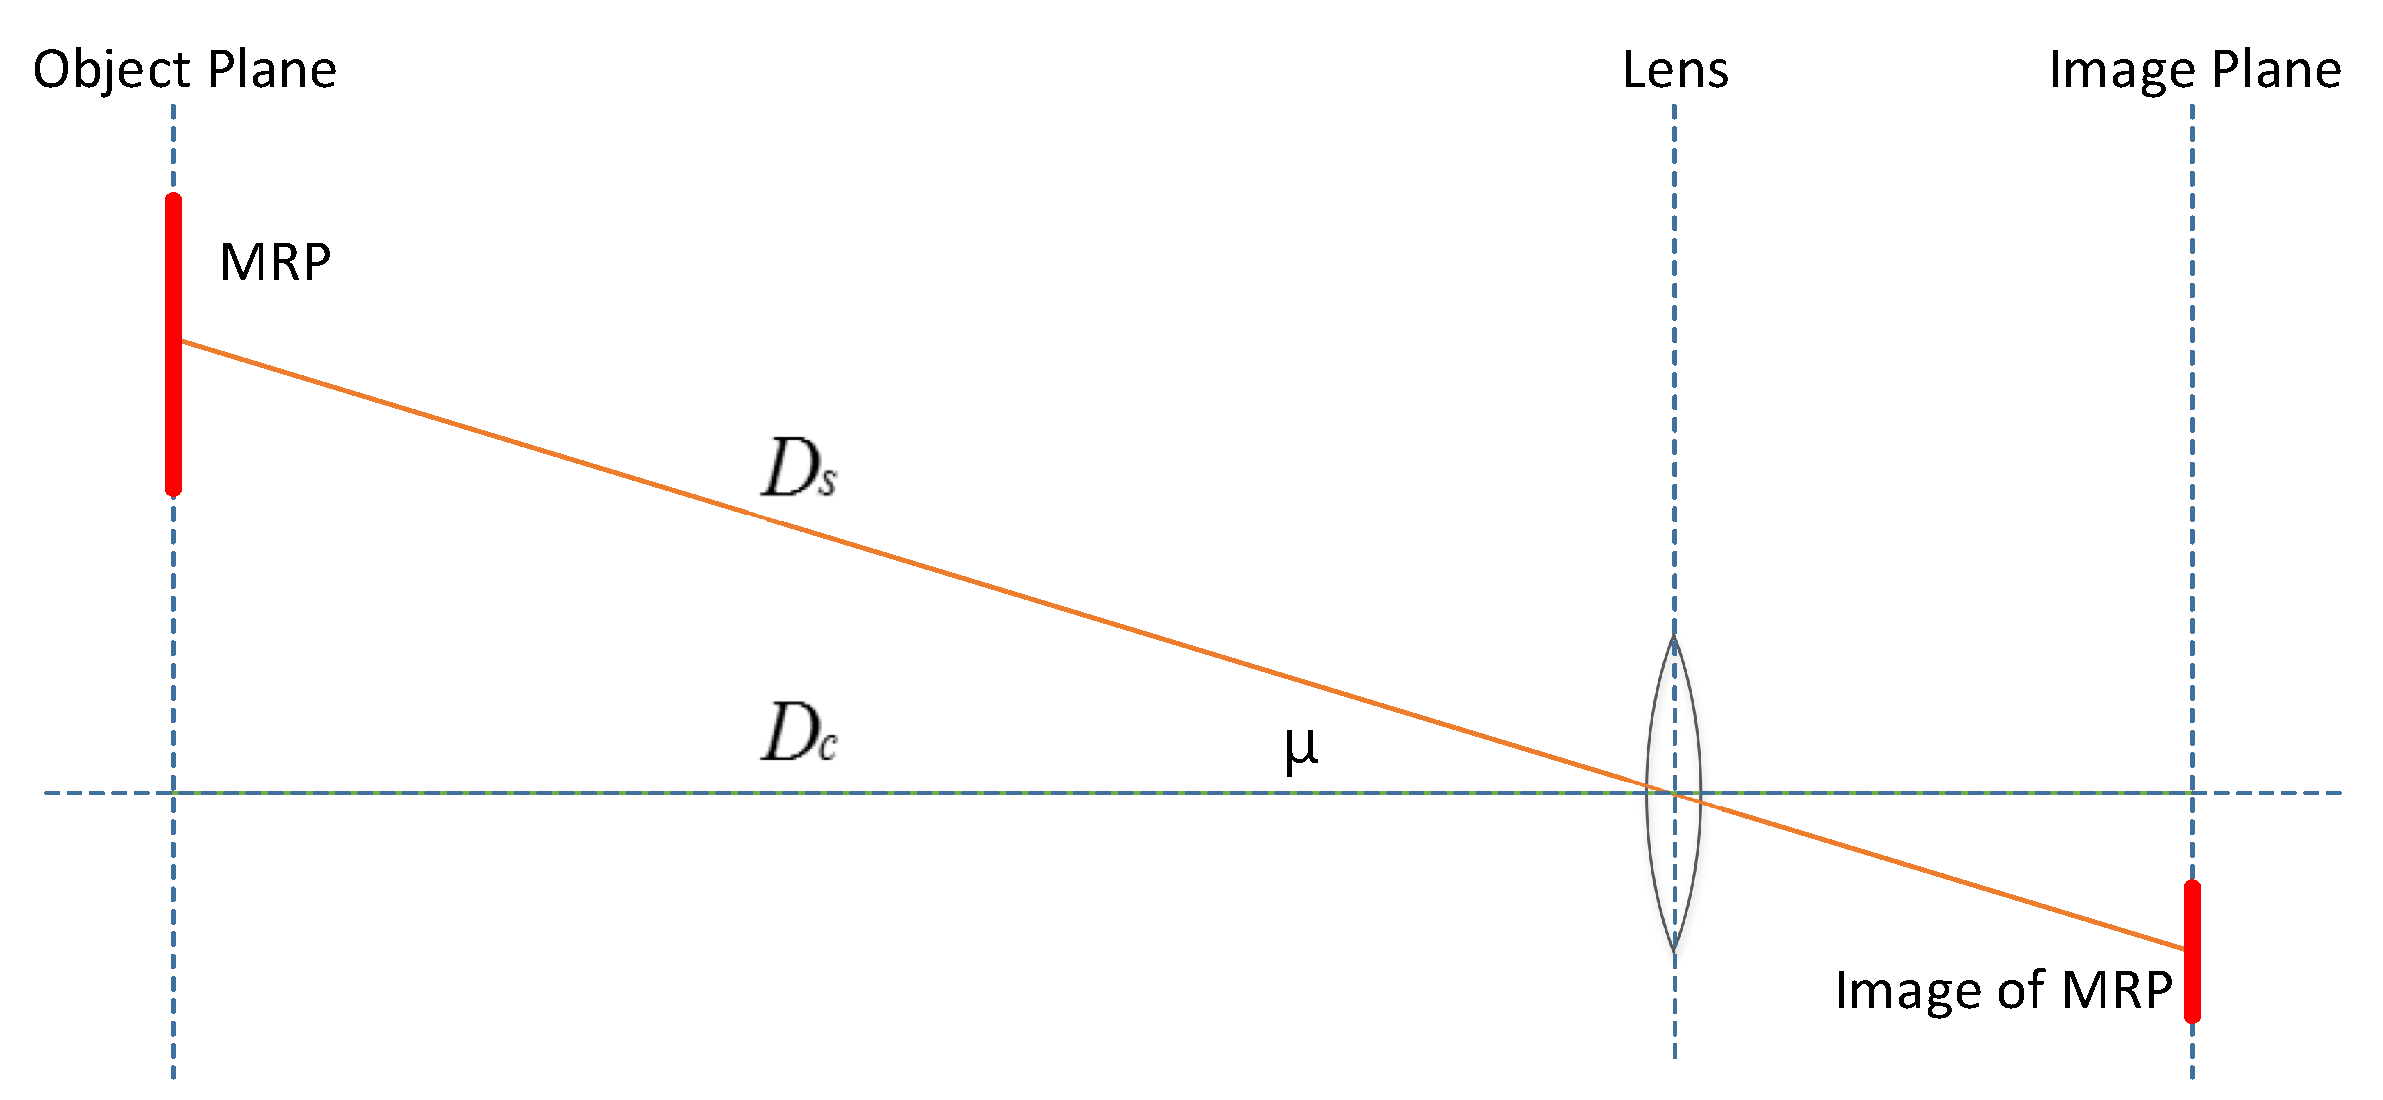
\includegraphics[width=3.5in]{fig/fig-distance-case2.eps}\\
%  \caption{MRP shifted on object plane.}\label{fig-distance-case2}
%\end{figure}
In this case, the MRP still facing toward the camera, but it is shifted by a distance on the direction perpendicular to the line between the MRP and the camera, as shown in Figure~\ref{fig-distance-case2}. We have found that if a MRP is shifted from the position directly facing the camera to the position up or down by a distance on the direction perpendicular to the line between the MRP and the camera, the projected image will remain the same size.

\begin{theorem}
The object has a fixed ratio to its projected image no matter how much of the distance it shifts on the direction perpendicular to the line between the MRP and the camera.
\end{theorem}

\begin{proof}
   Let the object plane be parallel to the image plane. We first assume the distance between the object plane and the lens (denoted as $D_o$) to be $x$ times of the distance between the lens and the image plane (denoted as $D_p$). In addition, we assume $O_\alpha$ to be originally facing directly to the camera and its projected image to be $P_\alpha$, as shown in Figure~\ref{fig-proof-projection}.
   Based on triangle rules, we have
    \[P_\alpha=D_p\tan(\alpha),\]
    \[O_\alpha=D_o\tan(\alpha)=x(D_p\tan(\alpha)).\] Consequently,
    \[O_\alpha=x(P_\alpha)\]

   Now assume that the object is shifted up by a distance. Without loss of generality, let the new location of the object to be $O_\beta$ and its projected image to be $P_\beta$.
   In case when $O_\alpha$ and $O_\beta$ do not overlap each other, as illustrated in Figure~\ref{fig-proof-projection}, we have
    \[P_\beta=D_p\tan(\alpha+\beta+\gamma)-D_p\tan(\alpha+\gamma)\]
    \[=D_p(\tan(\alpha+\beta+\gamma)-\tan(\alpha+\gamma)),\]
    \[O_\beta=D_o\tan(\alpha+\beta+\gamma)-D_o\tan(\alpha+\gamma)\]
    \[=xD_p(\tan(\alpha+\beta+\gamma)-\tan(\alpha+\gamma)).\] Consequently,
    \[O_\beta=x(P_\beta)\]

    As a result, we have
    \[\frac{O_\alpha}{O_\beta}=\frac{P_\alpha}{P_\beta}.\]
\end{proof}
\begin{wrapfigure}{r}{2.3in}
  \vspace{-20pt}
  \begin{center}
    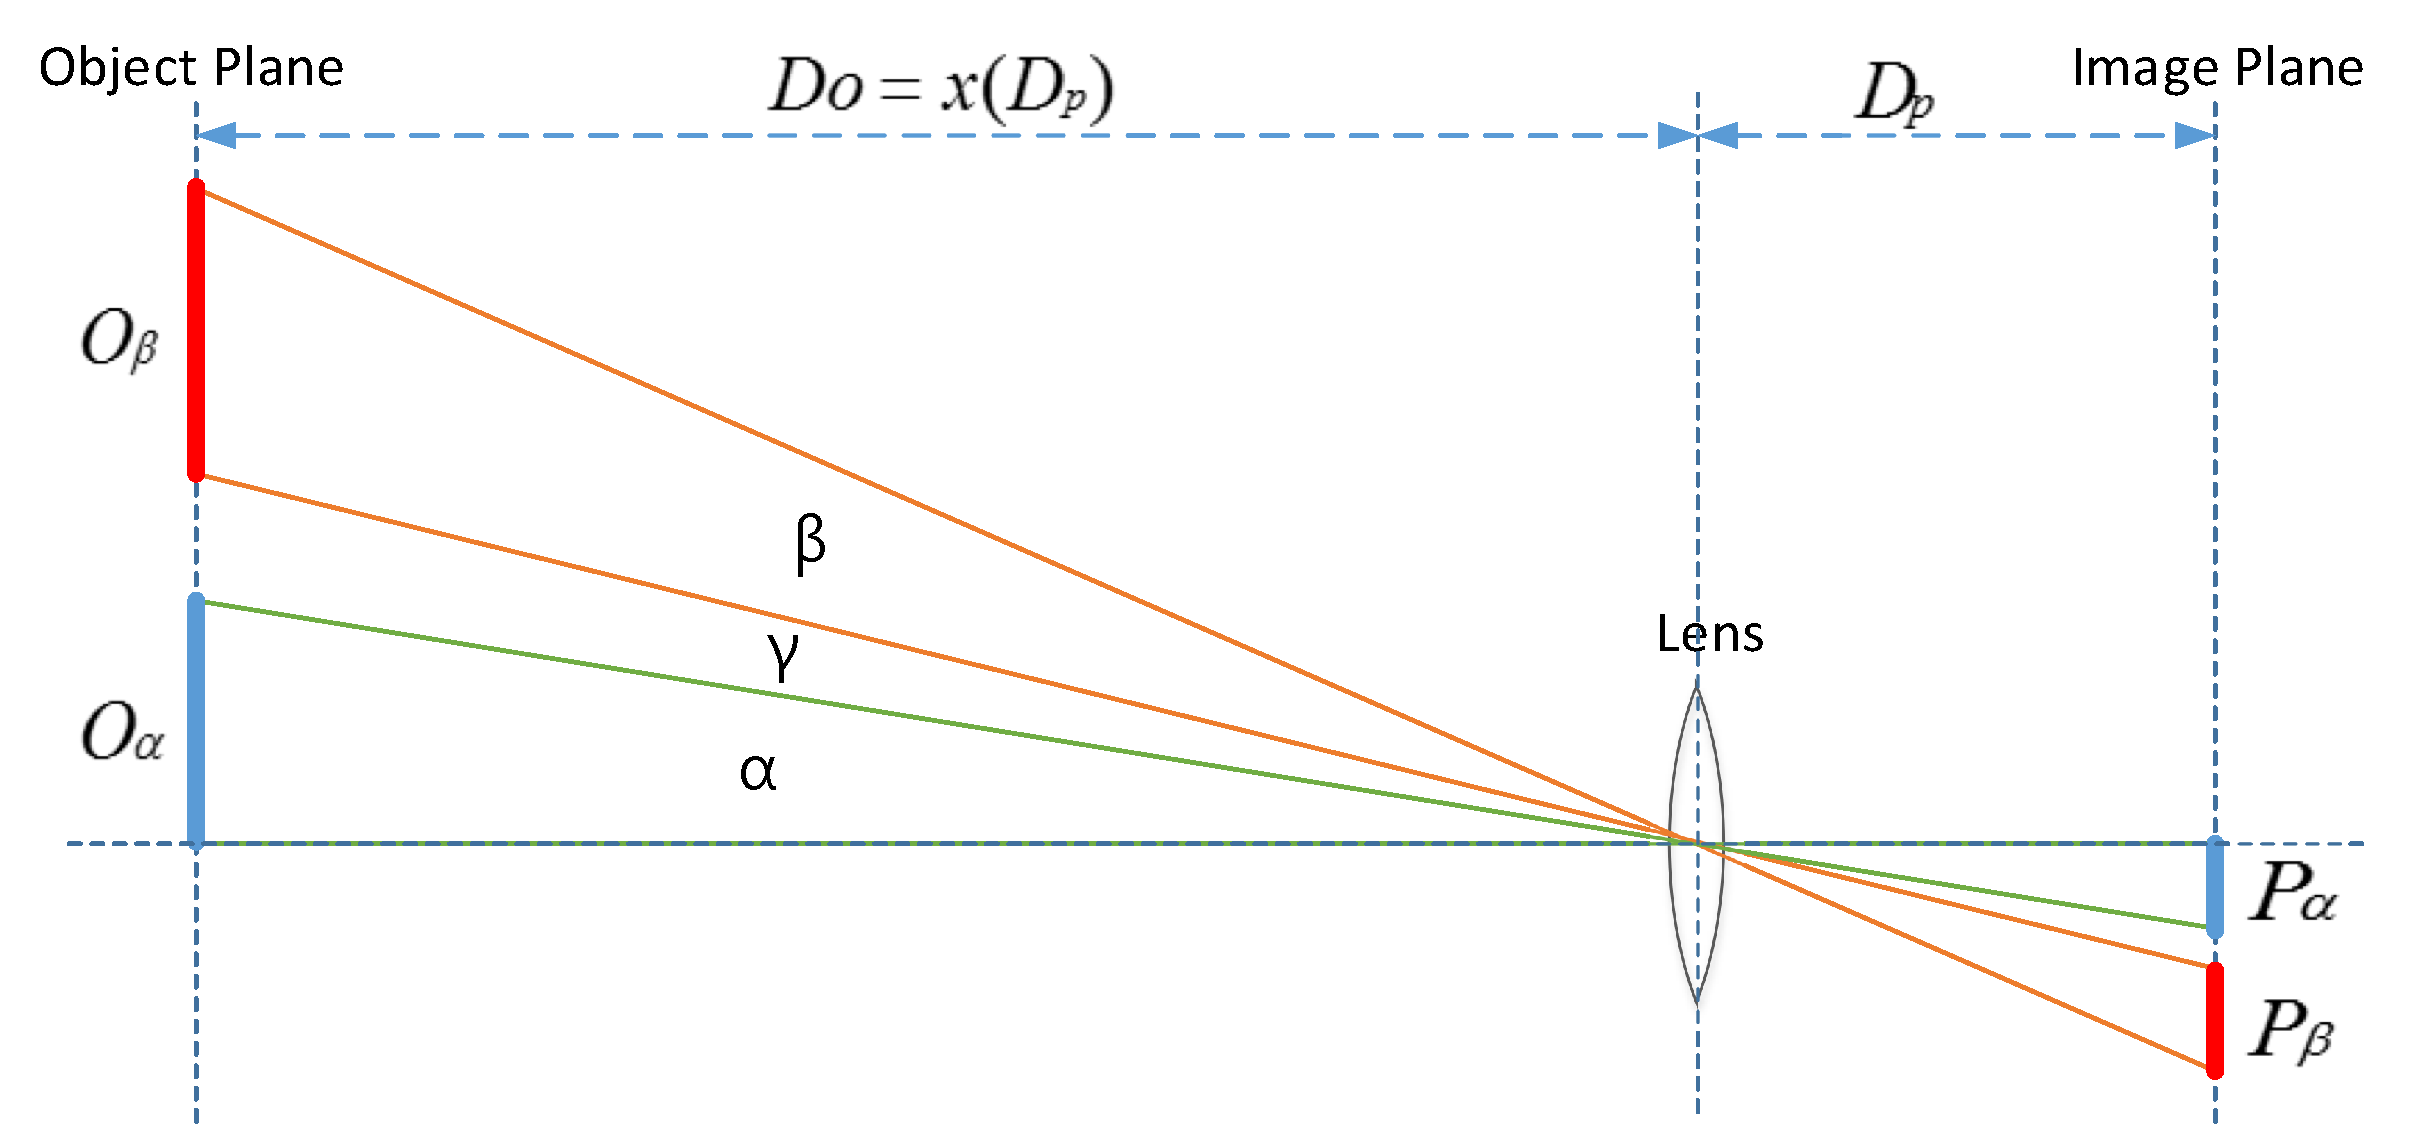
\includegraphics[width=2.5in]{fig/fig-proof-projection.eps}
  \end{center}
  \vspace{-20pt}
  \caption{Proof that object have a fixed ratio relationship with projecting image.}\label{fig-proof-projection}
  \vspace{-20pt}
\end{wrapfigure}
%\begin{figure}
%  \centering
%  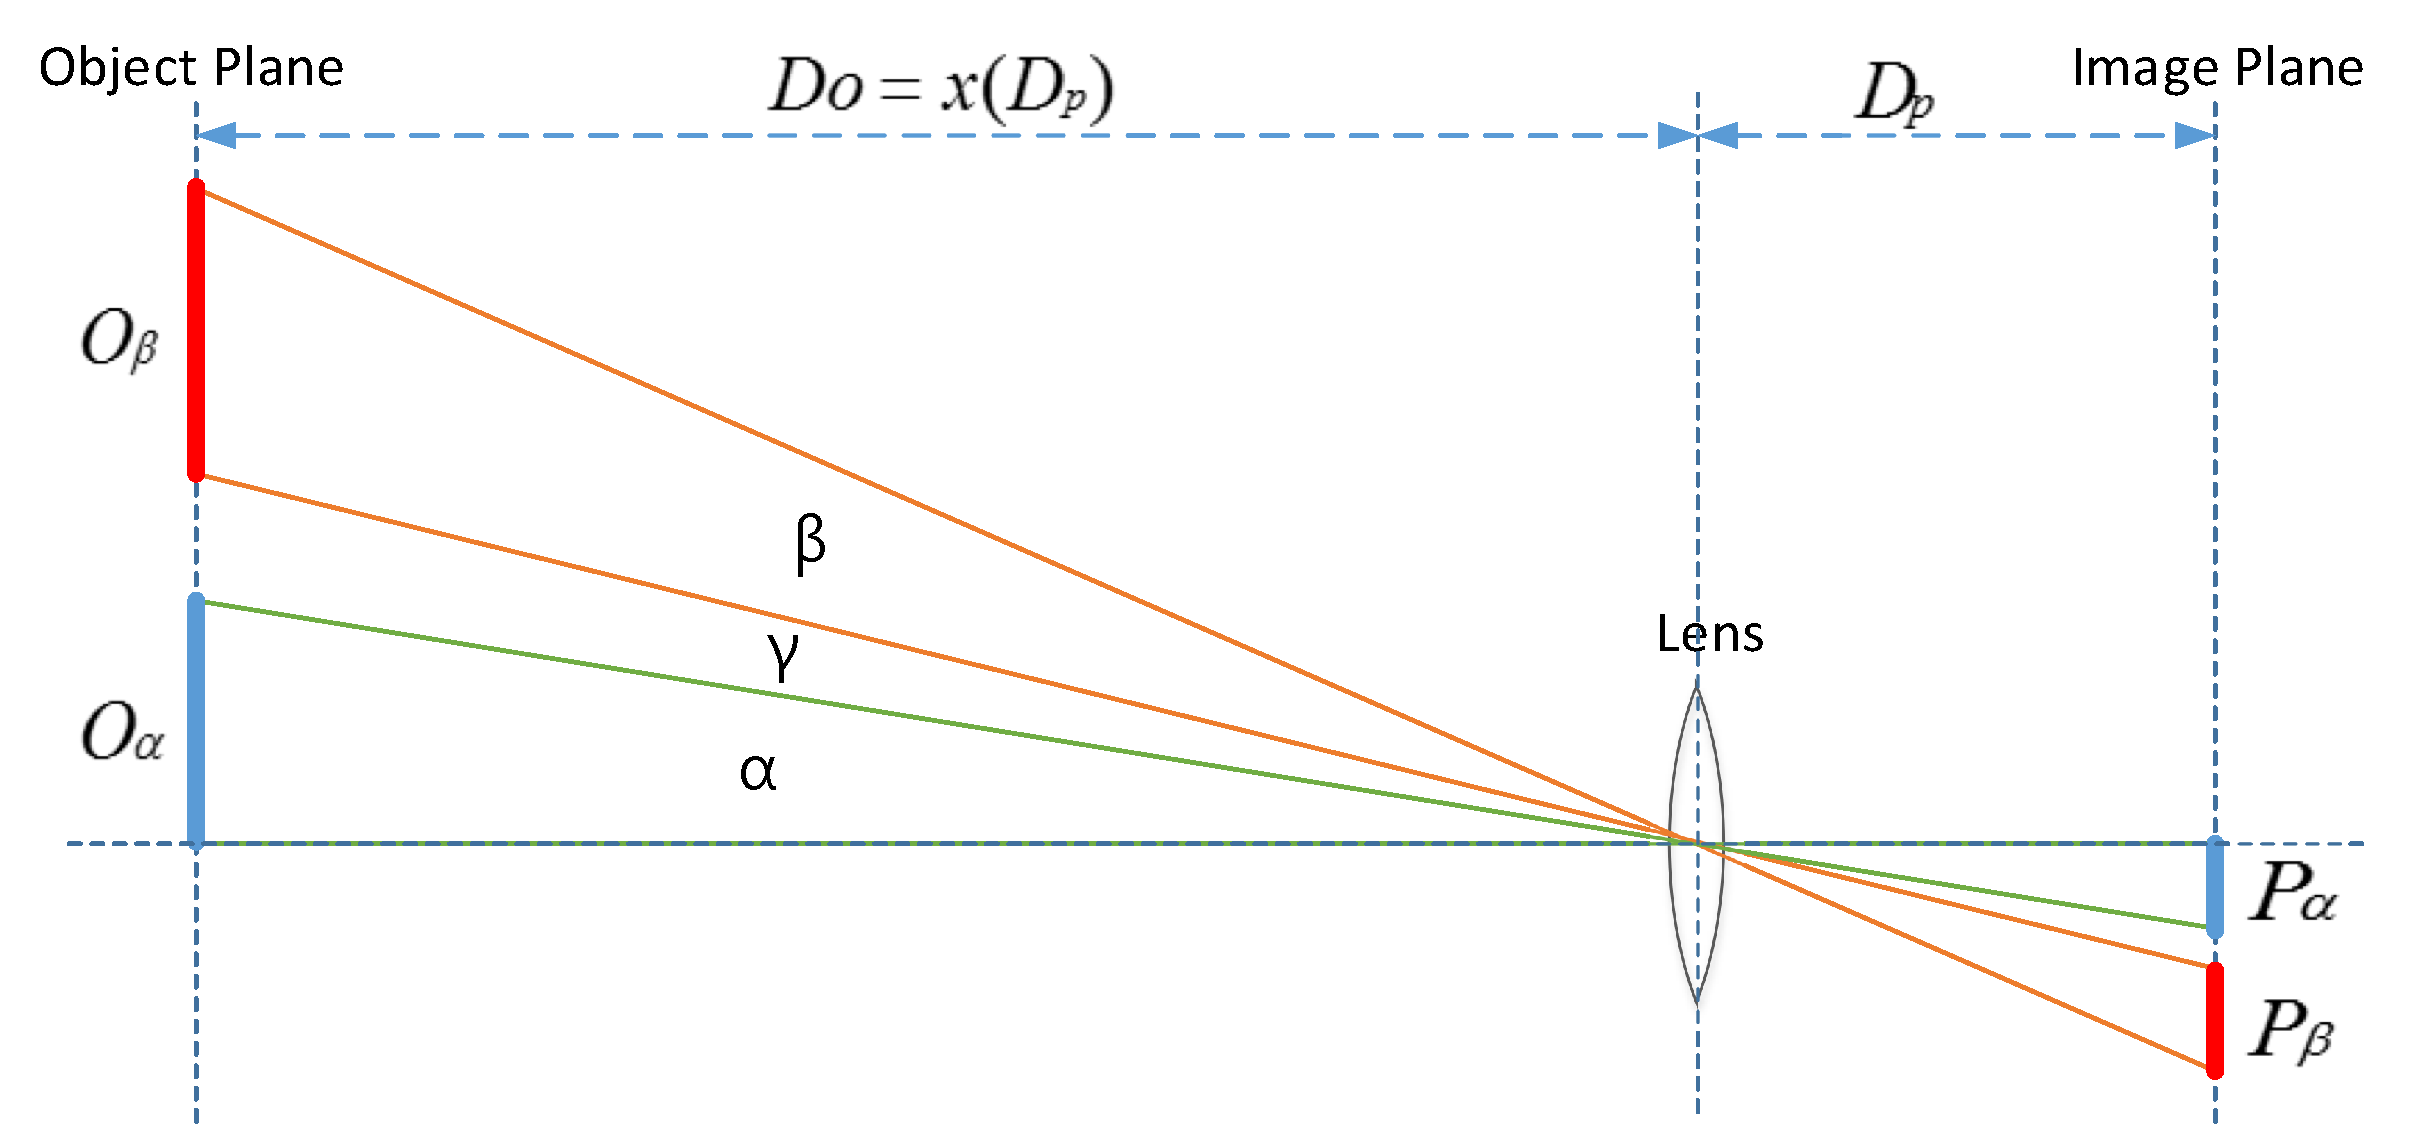
\includegraphics[width=3.5in]{fig/fig-proof-projection.eps}\\
%  \caption{Proof that object have a fixed ratio relationship with projecting image.}\label{fig-proof-projection}
%\end{figure}

Based on the above proof, we know that the distance between object plane and camera($D_c$) can be calculated directly from the size of the MRP projection.

However, the distance between two planes is not the actual distance between MRP and camera. In order to get the real distance from MRP to camera (denoted as \emph{Ds}), the additional required parameter is the angle between object plane and image plane, denoted as $\mu$. We can obtain $\mu$ by detecting the position of MRP in camera image, and then using the angle measurement method mentioned in seciton~\ref{sec-angle-measurement}. Once $\mu$ is obtained, according to the trigonometric functions, \emph{Ds} can be computed by equation:
\[Ds = \frac{{Dc}}{{\cos (\mu)}}\]

\subsubsection{Unparalleled Relationship}
\begin{wrapfigure}{r}{2.3in}
  \vspace{-20pt}
  \begin{center}
    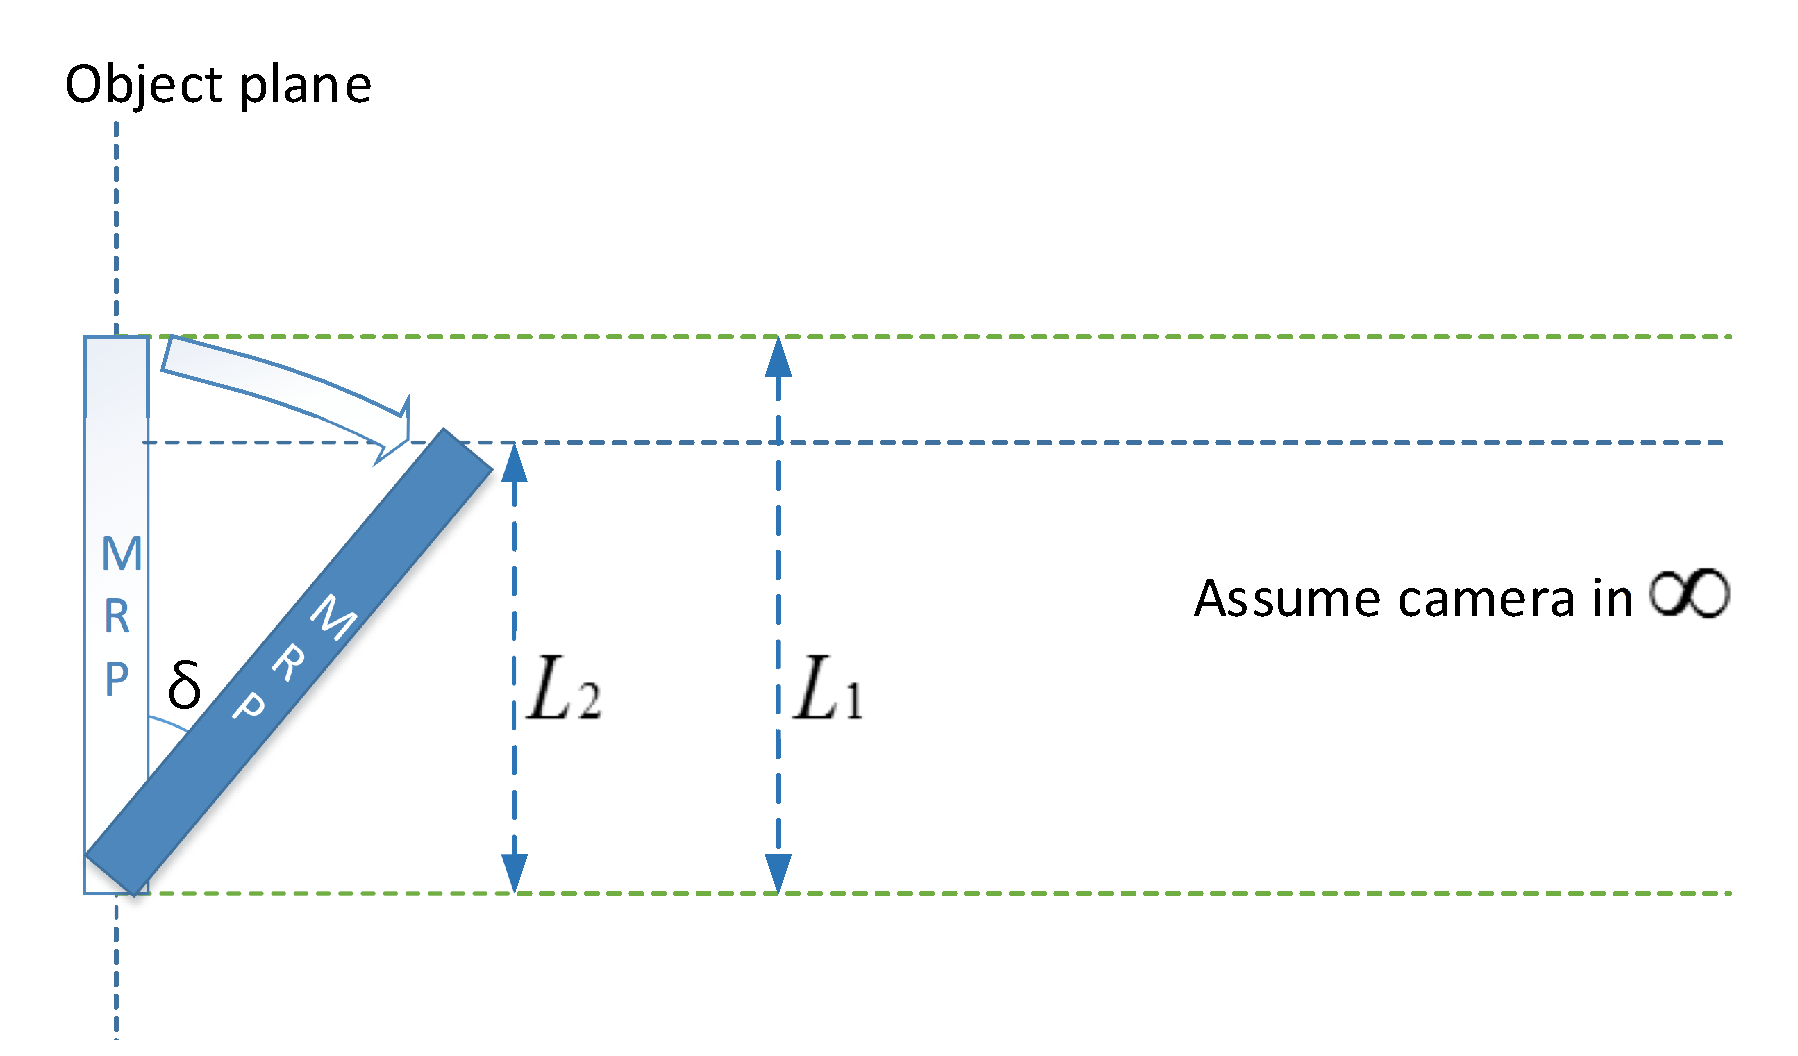
\includegraphics[width=2.5in]{fig/fig-distance-case3.eps}
  \end{center}
  \vspace{-20pt}
  \caption{Measure distance if MRP rotates.}\label{fig-distance-case3}
  \vspace{-20pt}
\end{wrapfigure}
%\begin{figure}
%  \centering
%  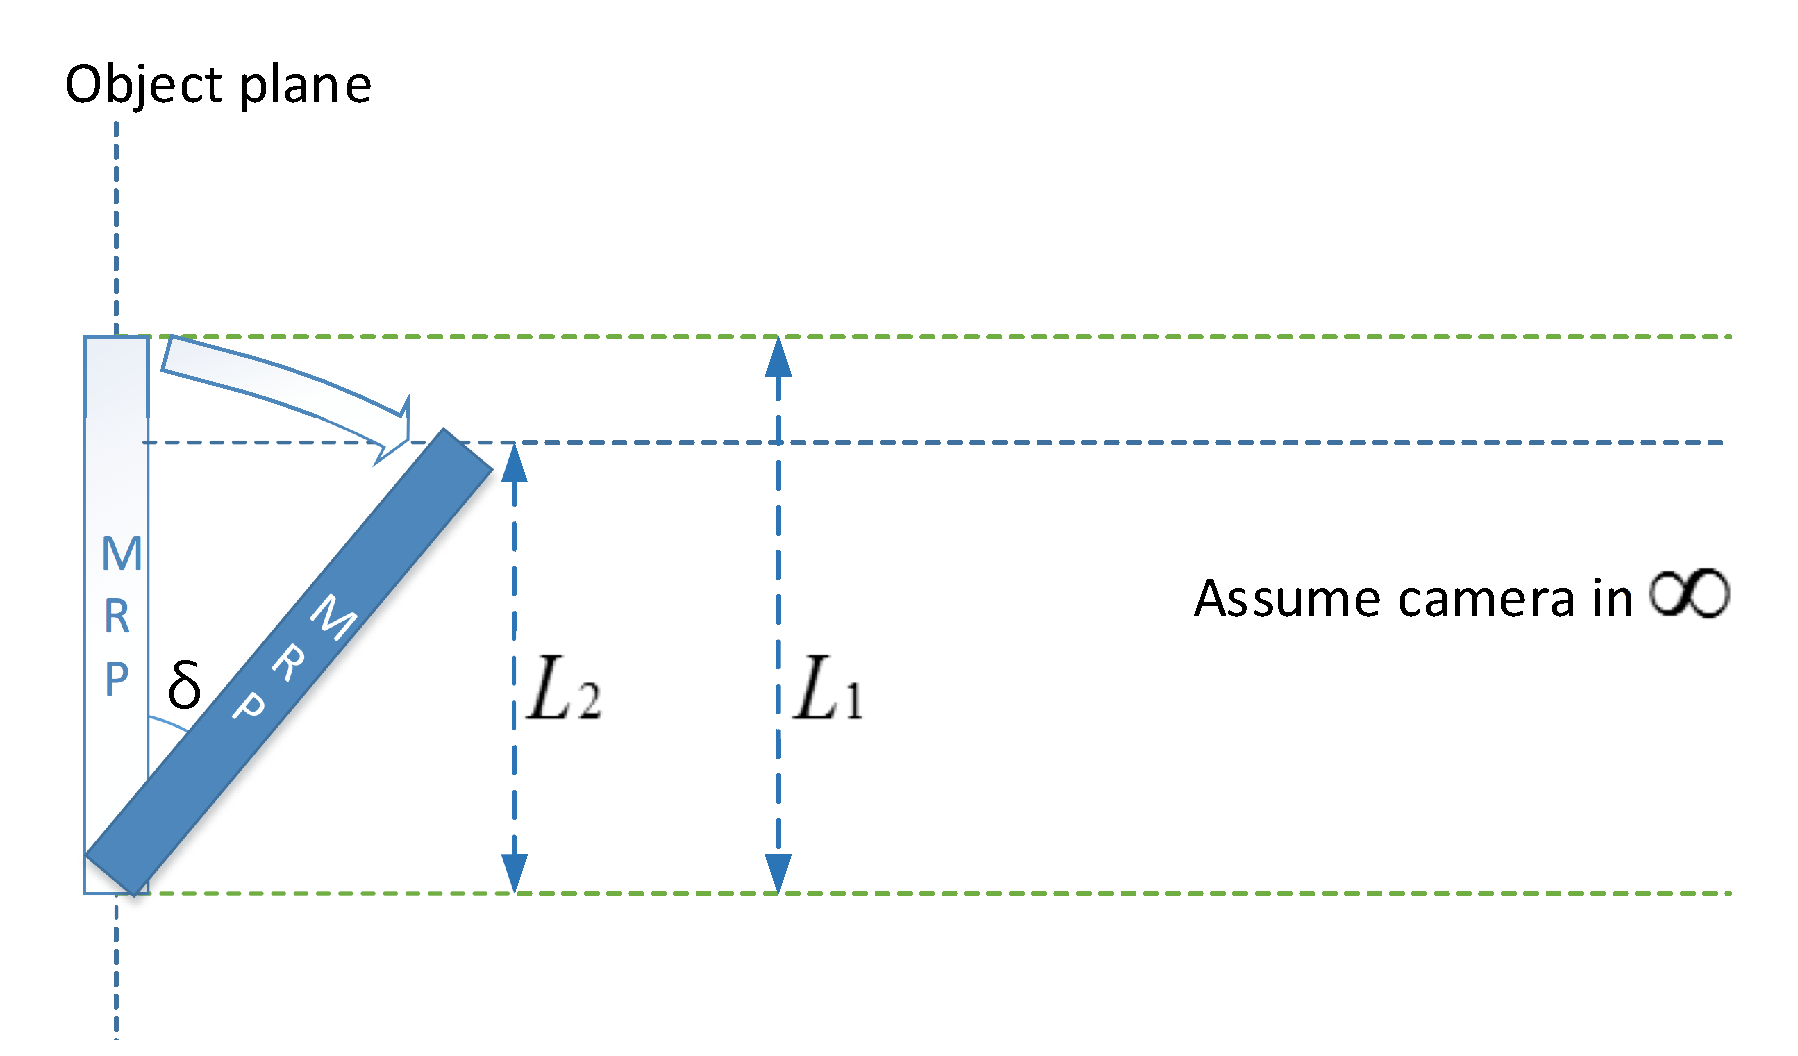
\includegraphics[width=3.3in]{fig/fig-distance-case3.eps}\\
%  \caption{Measure distance if MRP rotates.}\label{fig-distance-case3}
%\end{figure}
In this case. MRP is not facing toward object plane. We can imagine that it is like MRP is rotated for an angle as shown in Figure~\ref{fig-distance-case3}. In this case, the MRP size we measured \emph{$L_2$} will be smaller than true situation \emph{$L_1$}. For the convenience of calculation, we assume that camera lens is located at an infinite distance, then the MRP have an orthogonal projection relationship~\cite{wiki-projection} with the object plane as illustrated in Figure~\ref{fig-distance-case3}. The additional required parameter for this case is the angle between MRP and image plane (denoted as $\delta$).

$\delta$ can be obtained by calculating the difference of the orientation between MRP and camera. Unlike the orientation of MRP, which is fixed and known, the orientation of camera is dynamic. We use Android APIs to obtain the most recent orientation of camera. Readers interested in the Android APIs can refer to Android Developer Network~\cite{android-sensors-apis} for more information regarding Sensors APIs.

Once $\delta$ is obtained, according to the trigonometric functions, we can compensate and compute the real MRP image size \emph{$L_1$} using the equation below, then use \emph{$L_1$} to calculate the real distance between MRP and camera:
\[L_1 = \frac{{L_2}}{{\cos (\delta )}}\]

\subsection{Coordinate System Transformation}
Now we have the distance between camera and MRP, the orientation of camera, and the position of MRP in camera image. We can use these data to construct the vector \emph{$V_1$} that extends from the mobile device to MRP. Table~\ref{tb-comare-reference-system} summarizes the notation of different positions with respect to various reference systems.
\begin{table}
\begin{center}
    \begin{tabular}{ | l | l | l | }
    \hline
    Reference system & Position of MRP & Position of camera\\ \hline\hline
    Global reference system & $LLA_{MRP}$ & $LLA_{CAMERA}$\\ \hline
    MRP reference system & $(0,0,0)$ & $(x,y,z)$\\ \hline
    Mobile reference system & $(D,\zeta,\eta)$ & $(0,0,0)$\\
    spherical coordinate~\cite{wiki-spherical-coordinate-system} & & \\ \hline
    \end{tabular}
\end{center}
\caption{Comparison of various reference systems}\label{tb-comare-reference-system}
\end{table}


Notice that in the mobile reference system, $D$ denotes the radial distance of MRP from the camera, the $\zeta$ and $\eta$ denote the horizontal and vertical angular extent from the center of image to the position of image that MRP is located (See Figure~\ref{fig-mobile-reference-system}). For orientation angles, $u,v,w$ denote the pitch, roll, azimuth deviation between camera and MRP (See Figure~\ref{fig-orientation}).


\begin{figure*}[th!]
\begin{center}
 \begin{tabular}[t]{ccc}
    \begin{minipage}[t]{0.5\textwidth}
      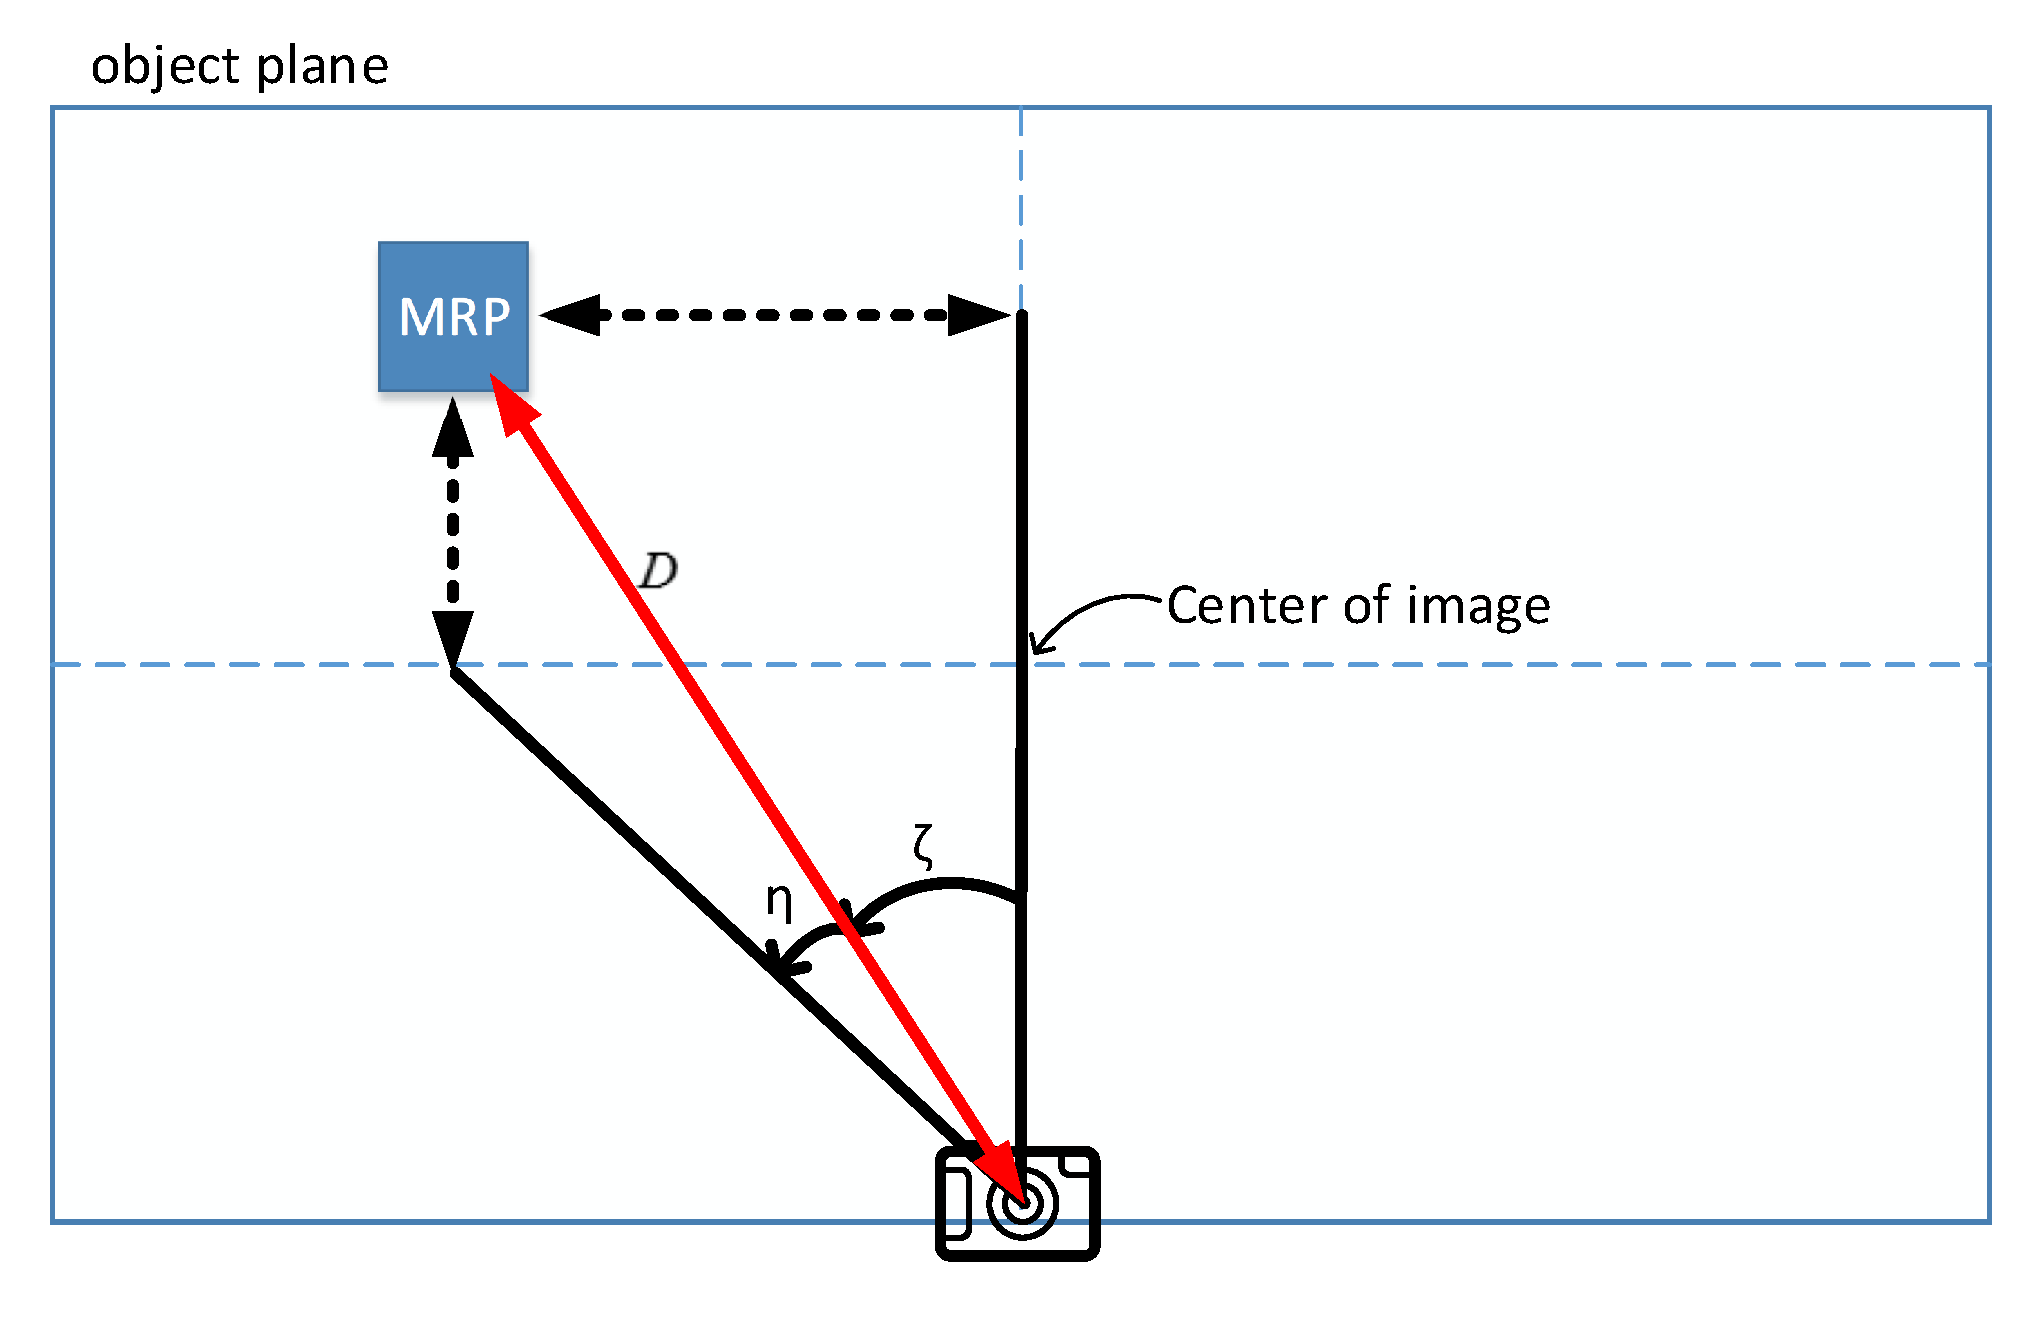
\includegraphics[width=\textwidth]{fig/fig-mobile-reference-system.eps}
      %\vspace*{-10pt}
      \caption{The mobile reference system.}\label{fig-mobile-reference-system}
    \end{minipage}
    \quad \quad
    \begin{minipage}[t]{0.5\textwidth}
      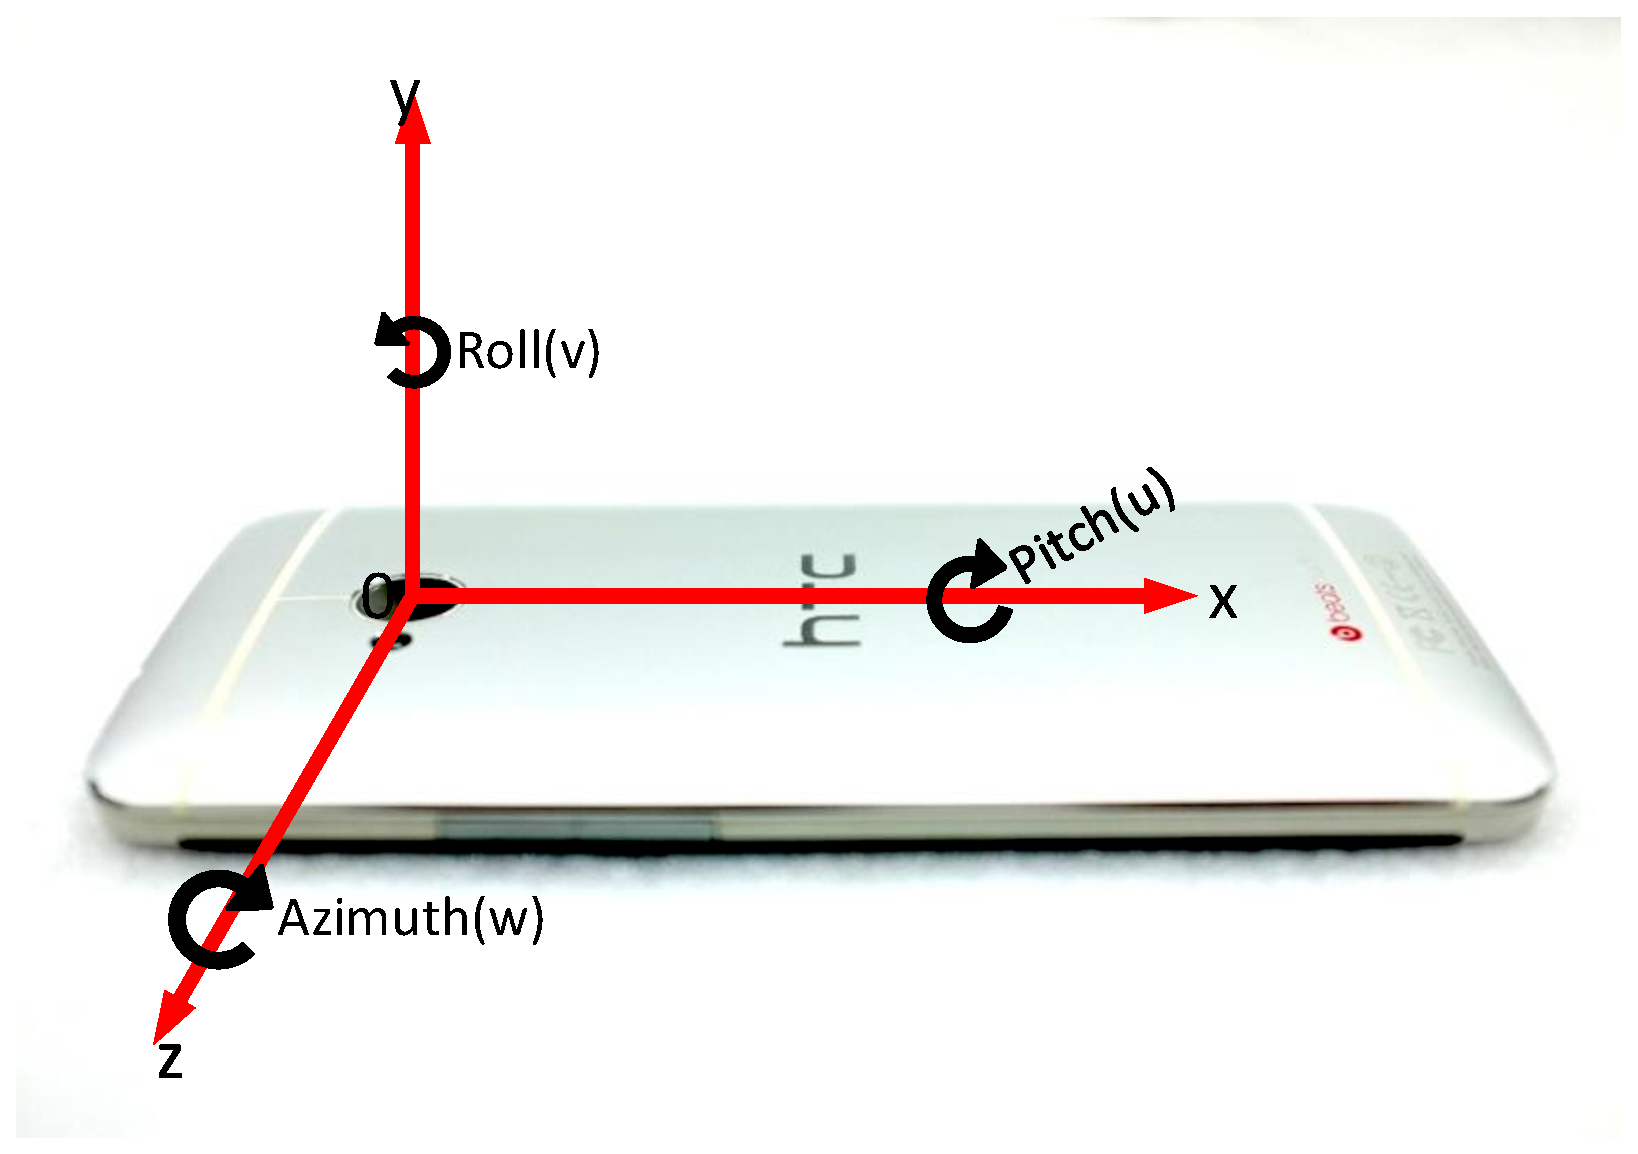
\includegraphics[width=\textwidth]{fig/fig-orientation.eps}
      %\vspace*{-10pt}
      \caption{The orientation of camera. Notice that we use the landscape mode.}\label{fig-orientation}
    \end{minipage}
  \end{tabular}
\end{center}
\end{figure*}

%\begin{figure}
%  \centering
%  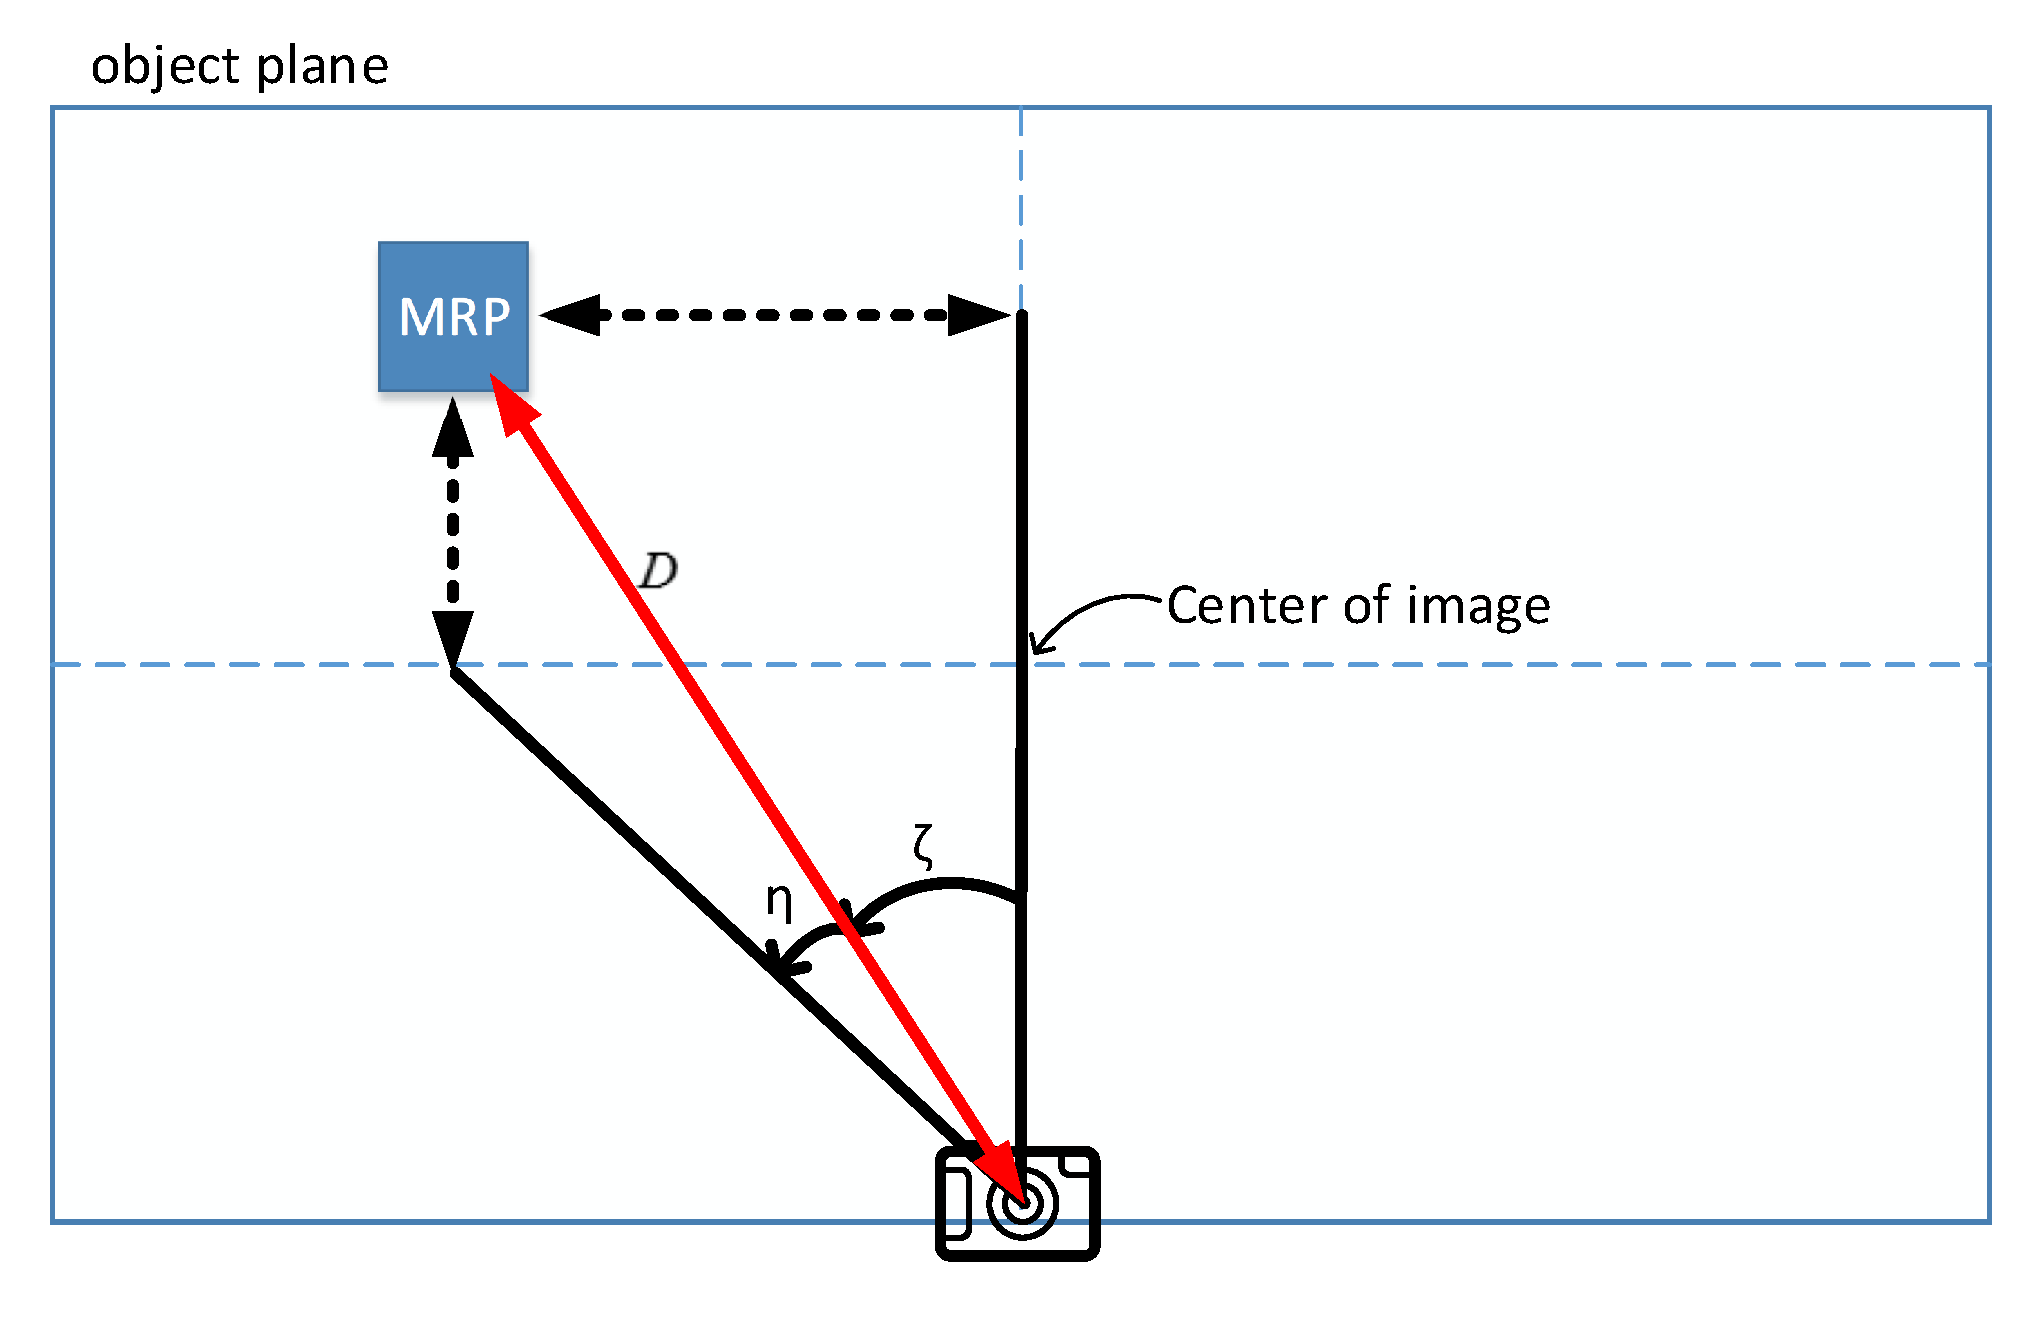
\includegraphics[width=3.3in]{fig/fig-mobile-reference-system.eps}\\
%  \caption{The mobile reference system.}\label{fig-mobile-reference-system}
%\end{figure}
%\begin{figure}
%  \centering
%  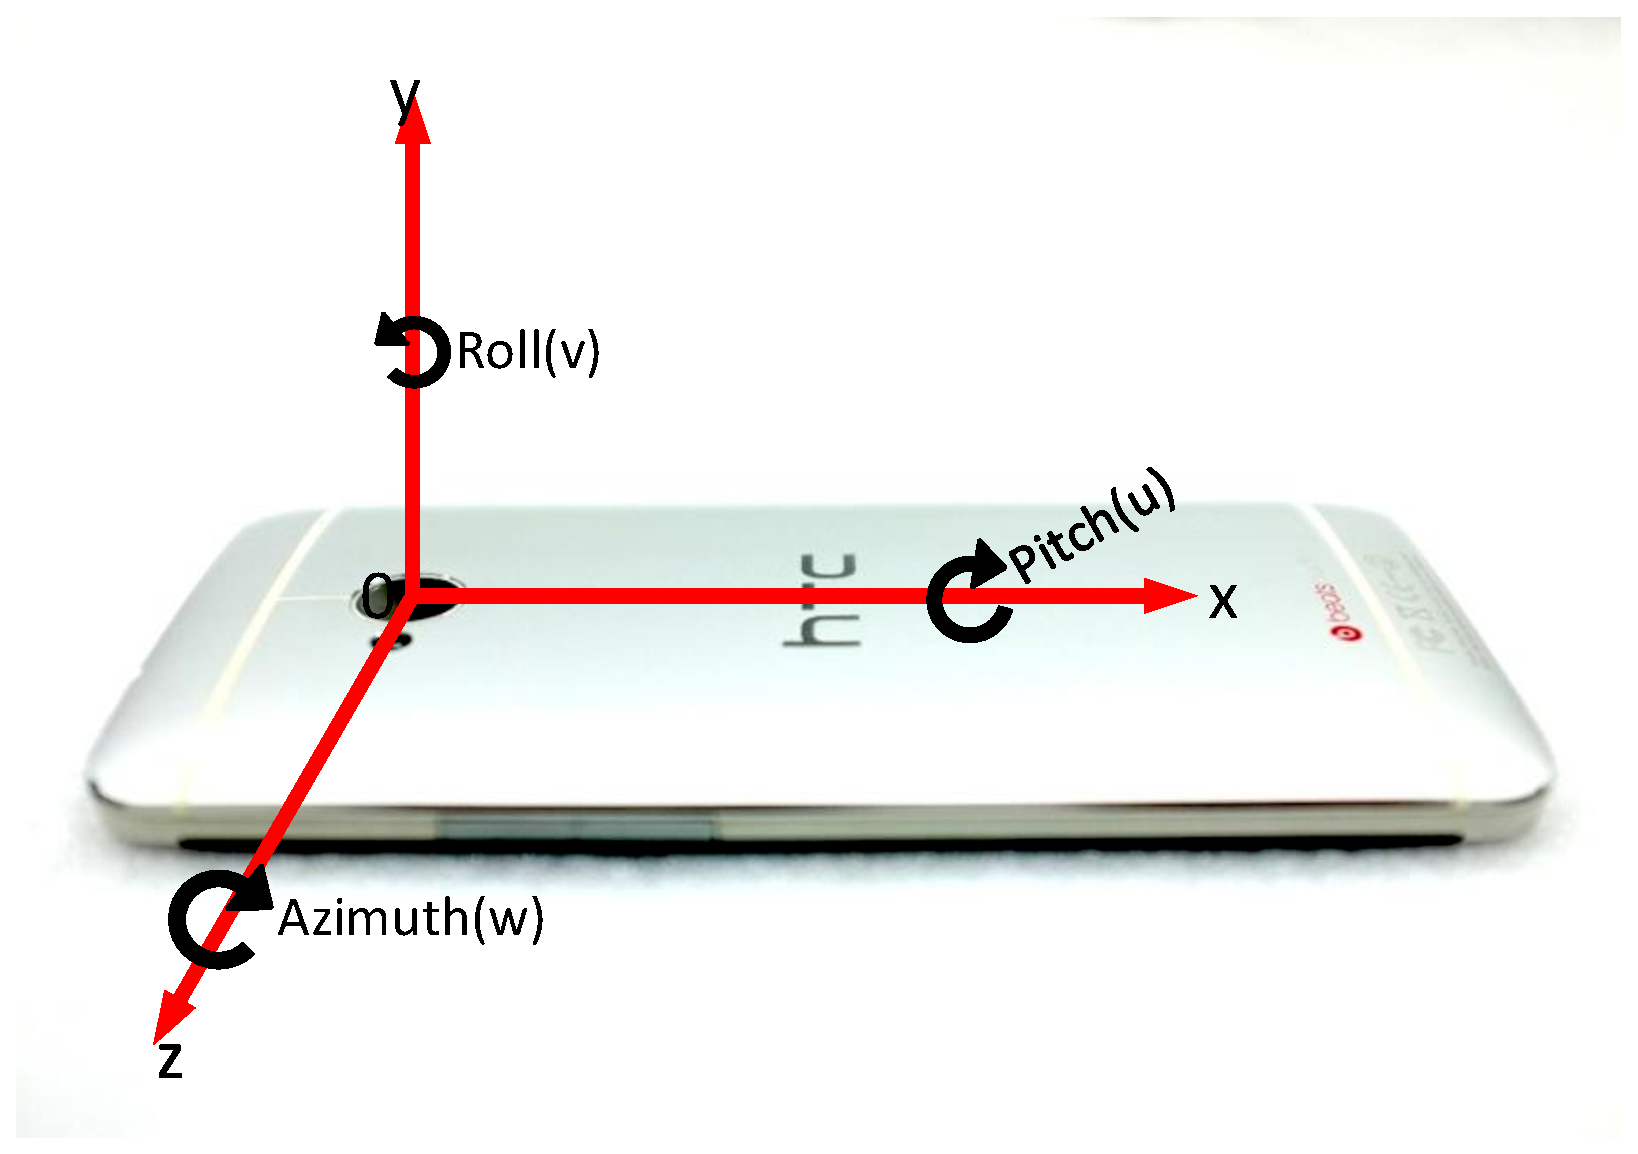
\includegraphics[width=3.2in]{fig/fig-orientation.eps}\\
%  \caption{The orientation of camera. Notice that we use the landscape mode.}\label{fig-orientation}
%\end{figure}
Note that the global reference position of MRP is known. Hence, if we transform \emph{$V_1$} to the MRP reference system, we can easily convert it to the global reference system.

In the following, we summarize the equations that transform \emph{$V_1$} to the MRP coordinate system:
\begin{enumerate}
  \item Rotate Y axis (roll angle)
\[\begin{array}{l}
x_1 = 0\\
y_1 = D\\
z_1 = 0
\end{array}\]
  \item Rotate X axis (pitch angle)
\[\begin{array}{l}
x_2 = x_1\\
y_2 = y_1 \times \cos (u-\eta)\\
z_2 = y_1 \times \sin (u-\eta)\\
\end{array}\]
  \item Rotate Z axis (azimuth angle)
\[\begin{array}{l}
x_3 =  - y_2 \times \sin (w-\zeta)\\
y_3 = y_2 \times \cos (w-\zeta)\\
z_3 = z_2
\end{array}\]
  \item Change values order compatible to global reference system Taiwan area(northern/eastern Hemisphere).
\[\begin{array}{l}
x =  - x_3\\
y =  - y_3\\
z = z_3
\end{array}\]
\end{enumerate}
\subsection{Hardware}
Our hardware environment is the HTC One Android smartphone, which has a build-in camera, gyroscope, geomagnetic field sensors and accelerometers.
Table~\ref{tb-key-hardware} shows the specification of key hardware components that we used in this project. Of course, our software can be deployed not only to the HTC One but also to any other Android devices.
\begin{table}
\begin{center}
    \begin{tabular}{ | l | l |}
    \hline
    Name & Specification \\ \hline\hline
    Camera & Max Picture Size: 2688 x 1520 \\
    & Max Video Size: 1920 x 1088 \\
    & Horizontal View Angle: 69.6 \\
    &Vertical View Angle: 43 \\ \hline
    Magnetic field sensor & Vendor: Asahi Kasei Microdevices \\
    & Model: AK8963 3-axis Magnetic field sensor \\ \hline
    Accelerometer & Vendor: BOSCH \\
    & Model: MBA250 3-axis Accelerometer \\ \hline
    Gyroscope & Vendor: ST Group Ltd. \\
    & Model: R3GD20 Gyroscope seosnr \\ \hline
    \end{tabular}
\end{center}
\caption{Key hardware components used in our visual-based positioning system.}\label{tb-key-hardware}
\end{table}

\subsection{Software}
Android is a Linux-based operating system designed primarily for touchscreen mobile devices such as smartphones and tablet computers. A developer survey conducted in May 2013 found that Android is the most popular platform for developers, It has been used by 71\% of the mobile developer population. Our experimental OS is Android version 4.1.2. The software is developed under The Eclipse IDE with The Android Developer Tools (ADT) plugin~\cite{developers2013adt}.
We choose ZXing~\cite{mackintosh2012zxing} as our QR-code decoding library. ZXing is an open-source, multi-format 1D/2D barcode image processing library implemented in Java.

\subsection{Magnetic Noise Issue}
\begin{wrapfigure}{r}{2.8in}
  \vspace{-40pt}
  \begin{center}
    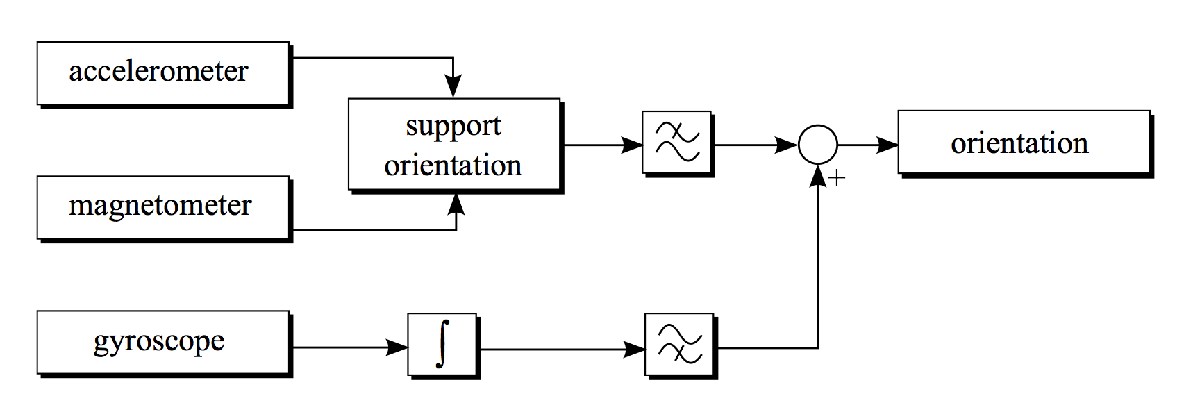
\includegraphics[width=2.8in]{fig/fig-complementary-filter.eps}
  \end{center}
  \vspace{-20pt}
  \caption{An overview of the complementary filter.}\label{fig-complementary-filter}
  \vspace{-20pt}
\end{wrapfigure}
%\begin{figure}
%  \centering
%  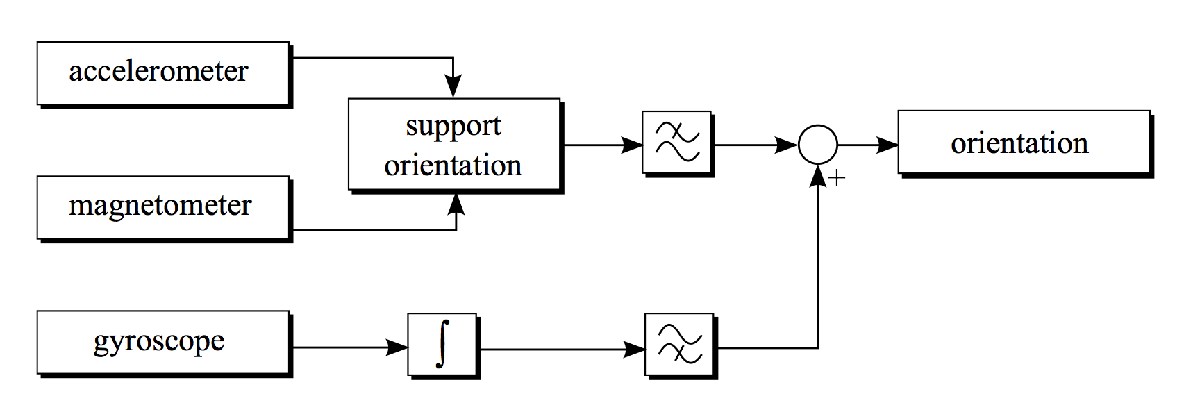
\includegraphics[width=3.3in]{fig/fig-complementary-filter.eps}\\
%  \caption{An overview of the complementary filter.}\label{fig-complementary-filter}
%\end{figure}
After our early system implementation, we found the issue of the magnetic noise. Magnetic noise is derived from device electronic parts and buildings. Section~\ref{complementary-filter} describes the complementary filter which can inhibit magnetic noise.

Complementary Filter for sensor fusion was proposed in~\cite{colton2007balance}. The gyroscope in the device is far more accurate and has a very short response time. Its downside is the dreaded gyro drift. The gyro provides the angular rotation speeds for all three axes. To get the actual orientation, those speed values need to be integrated over time.  This is done by multiplying the angular speeds with the time interval between the last and the current sensor output. This yields a rotation increment. The sum of all rotation increments yields the absolute orientation of the device. During this process small errors are introduced in each iteration. These small errors add up over time resulting in a constant slow rotation of the calculated orientation, called the gyro drift.

To avoid both gyro drift and noisy orientation, the gyroscope output is applied only for orientation changes in short time intervals, while the magnetometer/acceletometer data is used as the supporting information over long periods of time. This is equivalent to low-pass filtering of the accelerometer and magnetometer signals and high-pass filtering of the gyroscope signals. The overall sensor fusion and filtering are shown in Figure ~\ref{fig-complementary-filter}.

The sensors provide their data at (more or less) regular time intervals. Their values can be shown as signals in a graph with time as the x-axis, similar to an audio signal. The low-pass filtering of the noisy accelerometer/magnetometer signal (support orientation in figure~\ref{fig-complementary-filter}) are orientation angles averaged over time within a constant time window.

Later in the implementation, the low-pass filtering is accomplished by slowly introducing new values from the accelerometer/magnetometer to the absolute orientation:
\begin{verbatim}
// low-pass filtering: every time a new sensor value is available
// it is weighted with a factor and added to the absolute orientation
accMagOrientation = (1 - factor) * accMagOrientation + factor * newAccMagValue;
\end{verbatim}
The high-pass filtering of the integrated gyroscope data is done by replacing the filtered high-frequency component from accMagOrientation with the corresponding gyroscope orientation values:
\begin{verbatim}
fusedOrientation =
    (1 - factor) * newGyroValue    // high-frequency component
     + factor * newAccMagValue;    // low-frequency component
\end{verbatim}

Standard Complementary Filter is effective in electronic parts noise, but it is ineffective for inhibiting magnetic fields changes from buildings with reinforced concrete and steel structures. To solve magnetic fields changes, we prolong the complementary filter computing time intervals to grant the high-frequency values from gyroscope a higher impact. This change has a non-negligible effect in our experiments.

\subsection{Gyroscope Offset Issue}
One of the downsides of prolonging complementary filter computing time interval is that the effect of gyroscope offset becomes more significant. In order to alleviate the gyroscope offset problem, we sample offset values for a period of time and use their average value for compensation. This simple calibration method can reduce gyroscope offset from 2 seconds per degree to 45 seconds per degree.

\subsection{Startup Gyroscope Initial Values}
Another downside of prolonging complementary filter computing time interval is that the impact from standard e-compass (accelerometer and magnetometer) becomes minor. The gyroscope initial values should reduce the error from standard e-compass, so we use simple moving average filter (refer to Section~\ref{sma-filter}) to obtain better compass results for the startup gyroscope initial values. 